\chapter{体外膜氧合}

\section{前沿学术综述}

体外膜氧合(extracorporeal membrane
oxygenation,ECMO)是源于体外循环(cardiopulmonary
bypass,CPB)抢救重症患者生命的一项新技术,是一种持续体外生命支持的手段。体外膜氧合将血液从体内引流到体外,经人工膜肺氧合,氧合后的血液再重新通过静脉和(或)动脉灌注入体内,以维持机体各器官的灌注和氧合,对严重的可逆性呼吸和(或)循环衰竭患者进行长时间临时心肺支持,使心肺得以充分的休息,为抢救治疗和心肺功能的恢复赢得宝贵的时间。

体外膜氧合从20世纪70年代开始应用于临床,随着医疗技术、材料技术、机械技术的不断发展,其技术逐渐得到完善,并发症发生率不断下降,疗效改善,从而被更广泛地用于临床重症患者抢救和急救。体外膜氧合风险高、代价昂贵、操作管理技术和团队协作要求高,是代表医院,甚至一个地区、一个国家的重症患者救治水平的一项体外重要的生命支持技术。

\subsubsection{体外膜氧合的发展历史}

体外膜氧合是体外循环技术范围的扩大和延伸。1953年5月,Gibbon应用动脉氧合和灌注技术第一次成功实施直视下心脏手术,这种直视下心脏手术开展的体外循环具有划时代的意义,不但使心脏外科迅猛发展,同时也为体外生命支持手段谱写了新的篇章。在心脏手术期间快速建立的体外循环可以短期完全替代心肺功能,从而可以实施心内直视手术,从那时起就有了将此技术转化为一种生命支持抢救技术的想法。但当时存在一系列问题难以解决,主要包括肝素抗凝与出血的矛盾、生物材料组织相容性差、溶血、不能长时间进行膜肺氧合等。直到1972年,Hill报道使用3天的体外膜氧合成功抢救1例多发性创伤导致多器官损伤合并器官功能衰竭的患者
\protect\hyperlink{text00030.htmlux5cux23ch1-29}{\textsuperscript{{[}1{]}}}
。1975年,美国国立健康研究院主持了一项有关成人ARDS患者长时间体外循环支持抢救效果的多中心研究,这是历史上首次对一种研究终点为“死亡”的急性致死性疾病应用一种生命支持技术进行的前瞻性随机研究。该临床研究的设计和管理有很多问题,使得1979年发布的统计结果很不理想,但从其数据中仍然可以了解到,所有ARDS患者的总体死亡率为66%,严重ARDS的死亡率为90%
\protect\hyperlink{text00030.htmlux5cux23ch2-29}{\textsuperscript{{[}2{]}}}
。在当时条件下,如果由缺乏体外膜氧合经验的医院和医护团队,单纯应用股静脉股动脉体外膜氧合对患者进行呼吸支持1周,对严重ARDS患者的生存率提高没有帮助。随后对成人呼吸衰竭进行体外膜氧合终止了将近10年,但在新生儿呼吸衰竭治疗领域,体外膜氧合技术却首先取得了成功。1976年美国密西根大学医学院Bartlett等对一名因胎粪吸入综合征导致呼吸衰竭的女性弃婴施行体外膜氧合抢救成功
\protect\hyperlink{text00030.htmlux5cux23ch3-29}{\textsuperscript{{[}3{]}}}
。兴奋的医护人员将该婴儿命名为Esperanza,就是西班牙语“希望”的意思。该患者目前已经是一名健康快乐的母亲。上世纪80年代一些医院也陆续将体外膜氧合用于新生儿呼吸衰竭,并取得了较好的临床疗效。

体外膜氧合临床研究的开展和专业队伍的建设使体外膜氧合临床应用更加广泛,适应证也逐渐扩大。体外膜氧合逐渐为人们认识,一些医疗中心已组织专门医疗队伍进行体外膜氧合临床研究,体外膜氧合相关的材料、相应的方法和器械也在不断完善。1988年Bindslev等报告用肝素涂层新型膜肺建立体外膜氧合,可减少肝素用量和出血发生率
\protect\hyperlink{text00030.htmlux5cux23ch4-29}{\textsuperscript{{[}4{]}}}
。经皮插管方法可使体外膜氧合在短时间内建立,同时避免开胸和损伤大血管。1989年美国建立了“体外生命支持组织”(extracorporeal
life support
organization,ELSO),对世界范围内使用体外膜氧合的病例进行注册登记,便于统计、分析和总结体外膜氧合治疗的病例,进行体外膜氧合技术培训和推广。1993年Zwushenberrger等对7667例体外膜氧合治疗的急性呼吸衰竭患儿调查表明,其总生存率为81%,而如常规治疗生存率可能仅为20%
\protect\hyperlink{text00030.htmlux5cux23ch5-29}{\textsuperscript{{[}5{]}}}
。1994年另一项关于成人ARDS的RCT研究使用体外二氧化碳清除(extracorporeal
CO\textsubscript{2} removal,ECCO\textsubscript{2}
R)代替传统的体外膜氧合显示,与对照组相比,两组成人ARDS患者30天存活率分别为33%对比42%,两组间无显著统计学差异
\protect\hyperlink{text00030.htmlux5cux23ch6-29}{\textsuperscript{{[}6{]}}}
,但较70年代ARDS患者体外膜氧合治疗仅仅10%的存活率明显增加。1994年在英国召开体外膜氧合国际会议,对体外膜氧合技术和临床应用进行综合的总结和探讨,发现体外膜氧合对儿童特别是新生儿有很好的疗效,但对成人的效果不理想;对呼吸衰竭的效果较佳,对感染和心衰的效果较差。随着体外膜氧合技术的不断完善,双腔导管的出现使血管并发症进一步降低,另外也发展了各种转流方法,设备逐渐微型化,出现便携式体外膜氧合和无泵体外膜氧合等,其适应证因此而不断扩大。到2011年1月ELSO统计,全世界有4.5万患者进行了体外膜氧合治疗,总生存率为62%,其中100多个医疗中心用体外膜氧合对2.4万新生儿呼吸衰竭进行常规治疗,生存率为75%,一些有经验的中心新生儿呼吸衰竭存活率可达到90%。体外膜氧合治疗成人ARDS生存率在50%左右,对小儿和成人的循环支持的存活率较低,约在40%。体外膜氧合辅助下的心肺复苏患者支持治疗存活率也在30%左右。

\subsubsection{关于各种类型体外心肺支持的发展}

在体外膜氧合发展历史过程中,曾有不同的名称,在不同阶段源于体外循环技术也出现了不同的支持技术和手段,常用技术和手段名称列举如下。

\begin{center}
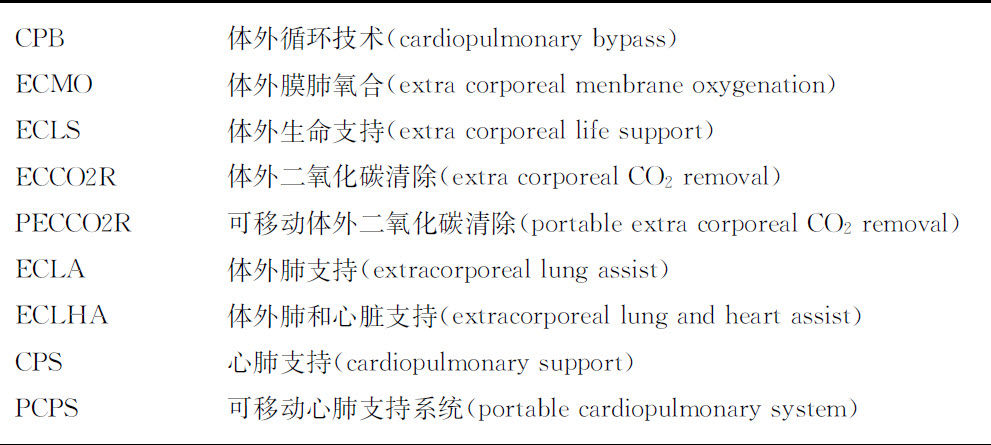
\includegraphics{./images/Image00279.jpg}
\end{center}

\begin{center}
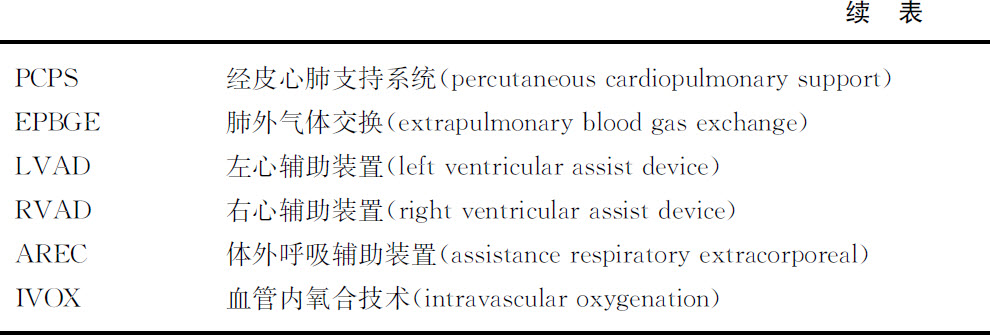
\includegraphics{./images/Image00280.jpg}
\end{center}

\subsubsection{体外膜氧合在成人急性呼吸衰竭的治疗进展}

体外膜氧合在儿童尤其是新生儿急性呼吸衰竭的治疗取得了较好的效果,但是在成人急性呼吸衰竭的治疗中未能获得良好的疗效,上个世纪70年代和90年代两项随机对照临床研究均未能显示体外膜氧合治疗能降低急性呼吸衰竭患者病死率
\protect\hyperlink{text00030.htmlux5cux23ch6-29}{\textsuperscript{{[}6{]}}}
\textsuperscript{,}
\protect\hyperlink{text00030.htmlux5cux23ch7-29}{\textsuperscript{{[}7{]}}}
。随着体外膜氧合材料的进步和技术的不断完善,管理水平的提高和规范化操作,使得体外膜氧合在成人急性呼吸衰竭患者的应用例数也逐年增加。

2009年Lancet发表英国完成的多中心随机对照临床研究(conventional
ventilation or ECMO for severe adult respiratory
failure,CESAR)通过与常规机械通气治疗比较,以期确定体外膜氧合治疗ARDS的安全性、治疗效果以及成本效益。研究共纳入180例重症ARDS患者,意向性分析体外膜氧合组纳入90例,常规治疗组纳入90例患者,实际接受体外膜氧合治疗者68例(75%)。体外膜氧合治疗者63%(57/90)无伤残存活至6个月,常规组为47%(41/87)
\protect\hyperlink{text00030.htmlux5cux23ch8-29}{\textsuperscript{{[}8{]}}}
。CESAR研究建议Murray评分>3.0或pH<7.20的成人可逆性、急性重症呼吸衰竭患者转往具备体外膜氧合治疗条件的医疗中心,可提高生存率并且无严重残障发生。虽然CESAR研究结果仍存在一些问题:①体外膜氧合治疗的患者都要转运到唯一的治疗中心,而常规治疗则在各分中心各自完成;②研究中“常规通气治疗”组没有统一的治疗方案;③体外膜氧合和常规机械通气两组在激素治疗、耐甲氧西林金黄色葡萄球菌(molecular
albumin recirculating
system)治疗、接受小潮气量低气道压通气策略治疗的人数以及时间差异均有显著的统计学意义。但是体外膜氧合具有机械通气所无法替代的特点,对于重症ARDS患者,CESAR研究为临床常规机械通气无明显改善的重症ARDS的治疗提供了最新的策略和相关依据。

体外膜氧合可支持重症ARDS患者气体交换,有可能降低ARDS患者病死率,并于2009甲型H1N1流感大流行期间用于治疗H1N1导致的ARDS。2009年H1N1的流行导致感染的重症患者迅速进展为急性重症呼吸衰竭,在澳大利亚和新西兰的多中心合作体外膜氧合治疗重症2009年甲型(H1N1)流感并发ARDS观察性研究中,用于68例使用机械通气和保护性肺开放治疗后仍有顽固性低氧血症和(或)高碳酸血症的ARDS患者,体外膜氧合平均支持时间10天,研究终点患者病死率为21%
\protect\hyperlink{text00030.htmlux5cux23ch9-29}{\textsuperscript{{[}9{]}}}
。2011年10月的《美国医学会杂志》(JAMA)发表英国皇家布朗普顿医院联合剑桥大学等多家研究机构实施的一项队列研究结果显示H1N1相关性ARDS患者,行体外膜氧合治疗可降低其住院病死率
\protect\hyperlink{text00030.htmlux5cux23ch10-29}{\textsuperscript{{[}10{]}}}
。研究纳入拟行体外膜氧合就诊与转诊的所有H1N1相关性ARDS患者作为研究对象,采用同期开展的、疑似或确诊的H1N1重症患者的纵向队列研究中的数据库,将体外膜氧合治疗患者和非体外膜氧合治疗患者进行匹配。主要转归指标为根据意向治疗原则的出院生存率,在80例意向体外膜氧合就诊患者中有69例(86.3%)患者行体外膜氧合治疗,其中22例(27.5%)在出院前死亡。从1756例常规治疗患者群中,采用个体匹配法、倾向评分匹配法和GenMatch匹配法分别确定了59、75和75例患者。研究结果显示与非体外膜氧合治疗患者相比体外膜氧合治疗患者的住院病死率均明显降低(\emph{P}
<0.01);敏感性分析(包括修改入选标准,限制非体外膜氧合就诊患者的治疗地点)显示,该项研究结果具有较高稳定性。体外膜氧合已经成为机械通气不能维持氧合的重症ARDS治疗救援措施之一
\protect\hyperlink{text00030.htmlux5cux23ch11-29}{\textsuperscript{{[}11{]}}}
,但是操作复杂,费用高,作为一线治疗措施尚未有充分明确的临床证据
\protect\hyperlink{text00030.htmlux5cux23ch12-29}{\textsuperscript{{[}12{]}}}
,仍需要更大规模临床研究进一步证实。

由于体外膜氧合并发症多,代价昂贵,是改善重症ARDS患者氧合、维持患者生命的临时救治手段,需待肺功能的恢复或下一步治疗,因此临床病例和治疗介入时机的选择尤为重要
\protect\hyperlink{text00030.htmlux5cux23ch13-29}{\textsuperscript{{[}13{]}}}
。目前认为体外膜氧合治疗的适应证是:①可逆性肺损伤导致的严重低氧血症(尽管高水平呼气末正压15~20cm
H\textsubscript{2}
O支持下氧合指数<80mmHg)至少6小时;②高条件机械通气支持下难以解决的呼吸性酸中毒(pH<7.15);③积极的最佳机械通气下难以接受的高气道平台压(根据患者理想体重调整潮气量气道平台压力>35~45cm
H\textsubscript{2}
O)。相对禁忌证包括:①高条件机械通气超过7天;②需要高吸入氧浓度支持(吸入氧浓度>0.8)超过7天;③不能建立血管通路;④其他任何造成患者难以从体外膜氧合获益的器官功能损害和临床情况,如不可逆的神经系统损害或难以治疗的转移性恶性肿瘤。绝对禁忌证为任何不能进行抗凝治疗的情况
\protect\hyperlink{text00030.htmlux5cux23ch11-29}{\textsuperscript{{[}11{]}}}
。

在ARDS的保护性通气策略中,减少潮气量是减少肺机械牵张性损害、改善患者预后的重要措施。当ARDS患者潮气量降至每千克理想体重4~6ml时,常出现通气不足及二氧化碳潴留,引起高碳酸血症及酸中毒。高碳酸血症具有抑制免疫反应的效应,在炎症反应早期有积极保护机体避免过度损害的效应,但严重的酸中毒可以导致血流动力学及免疫紊乱,长时间的高碳酸血症会导致感染扩散,加重器官损伤。

在保护性通气策略机械通气中的高碳酸血症可以使用人工辅助体外循环方式进行体外二氧化碳清除。自1972年第一例体外膜氧合临床应用以来,体外人工肺支持技术在不断改善,目前体外膜氧合已经作为ARDS时严重缺氧和高碳酸血症的拯救措施。由于体外膜氧合具有操作技术难,设备要求高等特点,且易出现溶血、凝血紊乱等副作用。为降低这些并发症的发生,另外一些操作简便新颖的ECLA技术开始在临床中应用,即无泵的动、静脉体外肺辅助系统(pump-less
arteriovenous extracorporeal lung assist
system,pECLA)或低流速泵驱动颈静脉二氧化碳清除系统,研究显示pECLA
相关的并发症发生率(12%~25%),显著低于传统的体外膜氧合(约50%)
\protect\hyperlink{text00030.htmlux5cux23ch14-29}{\textsuperscript{{[}14{]}}}
\textsuperscript{,}
\protect\hyperlink{text00030.htmlux5cux23ch15-29}{\textsuperscript{{[}15{]}}}
。

pECLA治疗ARDS的可行性在动物研究和临床研究中都得到了证实。这些研究都发现此系统能有效地清除二氧化碳,但对于系统改善氧输送的能力仍不十分明确。在肺泡灌洗复制猪急性肺损伤模型研究中,pECLA系统的血流量为心输出量的15%~21%,为1.3~1.9L/分,使用此系统后动脉血二氧化碳分压出现了显著性的降低(由71mmHg降至31mmHg),动脉血氧分压也出现了显著变化,但变化值较小(由64mmHg升至74mmHg),提供的最高氧输送量只占总氧耗量的17%。这些结果与成人ARDS患者的研究结果一致
\protect\hyperlink{text00030.htmlux5cux23ch16-29}{\textsuperscript{{[}16{]}}}
。虽然此系统改善氧合能力有限,但这些动物研究显示使用此系统后呼吸指标(如峰压、潮气量、呼吸频率)均得到改善。

pECLA的临床研究多为病例报告或回顾性研究。Being
T等回顾性地分析了90例不同病因的ARDS患者应用pECLA的情况,pECLA平均应用时间为5天。应用pECLA
2小时后,患者动脉血二氧化碳分压水平出现了显著性的改善(动脉血二氧化碳分压,60mmHg对比36mmHg);患者氧合亦出现了中度的增加(氧合指数58mmHg对比82mmHg),并持续改善至24小时(氧合指数101mmHg);从而可以下调呼吸机参数,降低了呼吸机相关肺损伤的风险;此研究中有24.4%患者出现相关并发症,主要表现为动脉置管侧下肢的缺血;最终pECLA治疗的ARDS患者病死率为58.8%,与存活者相比,病死者具有较大的年龄、较高的体重指数和使用pECLA前有较长的机械通气时间。这篇大样本的回顾性研究证实了此系统的安全性和有效性,且能保障肺保护性通气策略的实施,如降低潮气量和气道平台压等
\protect\hyperlink{text00030.htmlux5cux23ch15-29}{\textsuperscript{{[}15{]}}}
。近期上述研究单位完成了第一项关于pECLA的前瞻性观察性研究
\protect\hyperlink{text00030.htmlux5cux23ch14-29}{\textsuperscript{{[}14{]}}}
,该研究重新规范了pECLA的纳入和排除标准以及pECLA的临床操作技术。该研究结果同样证实了pECLA的安全性和有效性,患者病死率为49%,相关并发症的发生率可降低至11.9%,同时降低潮气量至4.4ml/kg亦可维持有效的通气和氧合,降低肺损伤的发生。2011年,在一家既往无pECLA经验的单位也发表了一篇13例重症ARDS患者的回顾性研究
\protect\hyperlink{text00030.htmlux5cux23ch17-29}{\textsuperscript{{[}17{]}}}
,该研究也同样证实了pECLA的安全性和有效性,病死率为54%,并发症发生率为23%。为进一步证实pECLA在ARDS患者治疗中的有效性,目前已有一篇随机对照研究(Clinical
Trials NCT 00538928)正在进行中,我们将期待此研究报告结果的发表。

pECLA的血液灌注主要由患者股动、静脉间的压差驱动,因此对于心输出量降低(心指数<2.7L/分/m\textsuperscript{2}
)或低血压(<70mmHg)的患者不适合应用
\protect\hyperlink{text00030.htmlux5cux23ch14-29}{\textsuperscript{{[}14{]}}}
,而且有导致下肢缺血的风险,因而限制了其临床应用。静脉-静脉二氧化碳体外清除系统(venovenous
CO\textsubscript{2} removal device,V\textsubscript{2}
CO\textsubscript{2}
R)是采用双腔颈内静脉置管连接低速泵驱动的体外膜肺装置,可以采用颈内静脉单针双腔导管以较低的流速进行二氧化碳清除,不存在动静脉分流,避免血流动力学的影响和动脉置管导致的下肢缺血。早在上世纪80年代Gattinoni就采用二氧化碳体外清除技术联合低频正压通气(low-frequency
positive pressure
ventilation,LFPPV)治疗43例预计病死率为90%的ARDS患者,体外膜氧合血流量(200~300)ml/分,72.8%患者肺功能改善,48.8%患者最终存活,但该研究采用常规的体外膜氧合设备进行,患者平均每日失血量达到(1800±850)ml,而且其中只有10例患者采用了双腔导管
\protect\hyperlink{text00030.htmlux5cux23ch18-29}{\textsuperscript{{[}18{]}}}
。其后二氧化碳体外清除技术治疗ARDS多为临床病例报告。新近的动物研究显示二氧化碳体外清除技术可以在降低潮气量和分钟通气量50%的情况下维持正常的水平
\protect\hyperlink{text00030.htmlux5cux23ch19-29}{\textsuperscript{{[}19{]}}}
,Batchinsky对7只镇静的、气管切开接受机械通气的猪进行泵驱动的静脉静脉二氧化碳体外清除治疗
\protect\hyperlink{text00030.htmlux5cux23ch19-29}{\textsuperscript{{[}19{]}}}
,利用15F的双腔颈内静脉置管连接Hemolung系统,逐步降低分钟通气量由5.6L/分下降到2.6L/分,Hemolung血流速为(447±5)ml/分可达到(72±1.2)ml/分的二氧化碳清除,且二氧化碳清除随体内动脉血二氧化碳分压的变化而变化。动物研究也显示二氧化碳体外清除技术流速较低,可采用枸橼酸体外抗凝技术
\protect\hyperlink{text00030.htmlux5cux23ch20-29}{\textsuperscript{{[}20{]}}}
,没有明显的失血和氧合器内凝血。

对于重症ARDS患者,pECLA是一种安全的、有效的、可操作性较强的体外肺辅助技术。它能有效地降低体内二氧化碳水平,辅助降低呼吸机参数,避免呼吸机相关肺损伤的发生。但目前仍需大规模的临床随机对照研究来进一步证实体外二氧化碳清除系统在肺保护实施和临床转归等方面的优势。

\subsubsection{体外膜氧合在心衰竭治疗中的进展}

体外膜氧合可以同时进行心肺支持,尤其是在急性心衰竭时可快速恢复合适的血流动力学,维持重要器官灌注和氧供,防治出现器官功能衰竭,给病变心脏恢复的时机或为心脏移植创造机会。体外膜氧合还可以避免大量血管活性药物造成的不良反应,如心律失常、多器官功能衰竭等,有望挽救患者生命。

体外膜氧合可用于心脏手术前心功能的维持,心脏术后低心排患者的心功能支持。研究显示,心脏术后出现低心排患者,如在合适的前负荷、大量血管活性药物和主动脉内球囊反搏支持下心输出量指数仍在2L/(分·m\textsuperscript{2}
)以下,行体外膜氧合支持患者生存率可达40%以上
\protect\hyperlink{text00030.htmlux5cux23ch21-29}{\textsuperscript{{[}21{]}}}
\textsuperscript{~}
\protect\hyperlink{text00030.htmlux5cux23ch23-29}{\textsuperscript{{[}23{]}}}
。虽然尚缺乏随机对照临床研究,但对于心脏术后严重低心排患者体外膜氧合是短期内心功能支持的重要手段。

心肌梗死的早期诊断和心血管介入技术发展,心肌梗死导致的急性心衰竭发生率已经较前下降,但合并急性心衰竭的急性心肌梗死患者病死率仍居高不下,即使再血管化治疗后病死率仍高达50%,早期给予体外膜氧合辅助有可能改善合并急性心衰竭的急性心肌梗死患者的预后。

爆发性心肌炎由于发病快、病情凶险,病死率高,体外膜氧合可能是早期循环支持的重要手段,为患者恢复和心脏移植创造时机。研究显示,虽然爆发性心肌炎病情进展迅速,但如果能获得早期机械循环支持,心肌得以休息反而利于病情恢复,12年远期生存率和并发症发生率优于急性心肌炎患者
\protect\hyperlink{text00030.htmlux5cux23ch24-29}{\textsuperscript{{[}24{]}}}
。

体外膜氧合治疗肺动脉高压和肺栓塞可以取得较好的效果,尤其是急性大块肺栓塞合并梗阻性休克的患者,体外膜氧合可以替代肺通气功能,在给空气时就能达到正常肺的氧合效果,可以减少肺血,维持心输出量,为手术或非手术方法解除栓塞提供生命支持
\protect\hyperlink{text00030.htmlux5cux23ch25-29}{\textsuperscript{{[}25{]}}}
。对于不可逆的肺动脉高压如原发性肺动脉高压,体外膜氧合仅用作肺移植或心肺联合移植前的过渡。

\subsubsection{体外膜氧合在心肺复苏方面的治疗进展}

在体外循环辅助的心肺复苏方面,体外膜氧合也能发挥一定的作用,新近研究显示体外膜氧合辅助的心肺复苏在60岁以下人群存活率达到30%,明显高于传统心肺复苏患者
\protect\hyperlink{text00030.htmlux5cux23ch26-29}{\textsuperscript{{[}26{]}}}
。

近年来心跳骤停(cardiac
arrest,CA)的救治取得了较大进展,自主循环恢复(restoration of
spontaneous
circulation)率可达40%~60%,但很多患者死亡发生于自主循环恢复后的24小时之内,主要原因为复苏后数小时心血管功能处于不稳定状态。心搏骤停时引起所有器官功能障碍;自主循环恢复后机体遭受二次打击,出现多器官功能障碍综合征,其中心脏能否维持泵血功能是患者能否生存的关键因素。随着心肺复苏进行,心肌缺血时间延长,反应性下降,最终心肌失去对各种治疗措施的反应性。对电除颤反应能力减弱,即使除颤成功,心肌处于“昏迷”或“冬眠”状态,仍不能有效泵血,导致复苏后循环功能不稳定,再次出现心跳骤停。

对心跳骤停患者来说,现代心肺脑复苏不仅是心脏的复苏,更重要的是脑复苏,恢复患者的神经系统功能为心肺脑复苏的最终目的。传统心肺脑复苏不能提供有效的心肌灌注,缺血心肌不能有效泵血,以至形成“低心输出量-心肌缺血加重-心跳骤停复发”的恶性循环。传统心肺脑复苏不能改善复苏结局的原因可能在于其心脑低灌注不足以维持器官功能。

体外膜氧合的建立最快可在数分钟内完成并用于心肺脑复苏,为心跳骤停的病人提供最快的心肺功能支持。与传统心肺脑复苏相比较,体外膜氧合可以提供足够心输出量,改善心、肺、脑等重要脏器的灌流,从而建立有效人工血液循环,保证心、脑及肺、肝、肾等重要生命器官灌流的同步性,为赢得抢救时机和提高抢救质量提供了又一途径。

但目前体外膜氧合辅助心肺复苏尚存有诸多方面的问题,如患者选择问题,现在尚无一种明确的标准可用以判定选择何种患者进行体外膜氧合辅助心肺复苏可以获得最佳的治疗作用。动、静脉插管是建立体外膜氧合的第一步,对整个体外膜氧合复苏过程具有举足轻重的作用。操作者必须迅速、顺利地完成动、静脉导管置入,否则体外膜氧合将无从建立,或延误时机而导致复苏失败。随着体外膜氧合辅助心肺复苏应用推广及技术本身的发展,越来越多不同专业的医务人员将参与到这项工作中来,包括重症医学科、心胸外科、心内科、急诊室、麻醉科及其他许多科室的医生。为了迅速、成功地建立并完成体外膜氧合辅助复苏,要求各个专业人员在工作中密切配合。

\subsubsection{体外膜氧合在其他适应证的治疗进展}

随着体外膜氧合技术的不断完善,其适应证也在不断地扩大,并取得了良好的临床预后。如一些急性中毒患者可因循环和呼吸衰竭而迅即死亡,通过体外膜氧合有效地呼吸循环支持同时通过人工肾、人工肝等技术帮助毒物的排除,可能挽救此类患者的生命
\protect\hyperlink{text00030.htmlux5cux23ch27-29}{\textsuperscript{{[}27{]}}}
\textsuperscript{,}
\protect\hyperlink{text00030.htmlux5cux23ch28-29}{\textsuperscript{{[}28{]}}}
。

由于感染性休克的患者血液中存在大量的细菌或病毒,释放毒素造成全身细胞功能障碍,细胞对氧利用力降低而处于缺氧状态;同时血管扩张、外周阻力降低、血压下降、组织灌注不足、细胞缺氧、大量乳酸产生,一些毒素可直接对心肌造成损伤,使心排量降低。以往的经验认为体外膜氧合对感染性休克的作用有限,为体外膜氧合的相对禁忌证,但多年的实践证明高流量体外膜氧合可有效地对此类患者进行支持,有利于患者的早日康复
\protect\hyperlink{text00030.htmlux5cux23ch29-29}{\textsuperscript{{[}29{]}}}
\textsuperscript{,}
\protect\hyperlink{text00030.htmlux5cux23ch30-29}{\textsuperscript{{[}30{]}}}
。

\subsubsection{我国体外膜氧合临床应用的进展}

我国体外膜氧合的工作起步较晚。1993年北京阜外医院成功地用体外膜氧合抢救一例心脏手术后急性呼吸功能衰竭的老年患者,但此患者的救治并非真正意义上的体外膜氧合,采用的是开放式膜肺进行转流,患者在体外膜氧合期间全程采用肝素抗凝,激活全血凝血时间(ACT)大于480s。上世纪末广东中山市医院也开始体外膜氧合的临床应用,此后在多家医院得到开展。本世纪初,北京和上海一些医院如阜外医院、安贞医院、上海胸科医院等相继开展体外膜氧合工作,治疗应用范围很广,如体外循环后的心肺支持、烧伤后ARDS的治疗、在体外膜氧合支持双肺停止呼吸情况下对肺泡蛋白沉着症行支气管肺泡灌洗术、肺移植后的支持、肺栓塞开胸取栓和心脏移植的前期准备等。到2008年为止全国有43家医院可开展体外膜氧合,总例数为185例,涉及范围主要在心脏外科术后。阜外医院体外膜氧合的循环支持临床疗效突出,报道出院生存率达57%
\protect\hyperlink{text00030.htmlux5cux23ch31-29}{\textsuperscript{{[}31{]}}}
。

H1N1的爆发流行促进体外膜氧合临床应用的快速进展,国内多家医院开展体外膜氧合治疗H1N1相关性ARDS,取得良好的效果。世界上各国体外膜氧合治疗ARDS的经验使国内体外膜氧合的发展获得了新的机遇,相信在不远的将来,随着国家经济不断发展,体外膜氧合治疗技术不断成熟,我国体外膜氧合辅助心肺支持将步入快速增长的发展阶段,更好更多地为患者服务。但是体外膜氧合并非常规治疗手段,操作复杂,适应证选择和临床管理均需要专业团队进行,风险高,费用高,因此体外膜氧合在我国发展过程中需要不断学习,建立专业团队,进行正规培训,建立国内专业数据库
\protect\hyperlink{text00030.htmlux5cux23ch32-29}{\textsuperscript{{[}32{]}}}
。

体外膜氧合可以在一段时间内维持患者的心肺功能,从而为治疗争取时间,挽救部分病人的生命,是一个很重要的支持治疗手段,但它不是病因治疗,如果患者器官功能短期内不能恢复或无其他治疗方法如器官移植,体外膜氧合虽可以延长患者的生存时间,但病人仍会死于原发疾病或体外膜氧合所导致的并发症。只要能慎选真正需要的病人,尽早临床使用,并在训练有素精诚合作的团队强力支持下,相信体外膜氧合必能帮助更多的患者度过最危急的阶段。体外膜氧合技术复杂,人力、物力、财力消耗大,持续时间长、涉及方面多、远期效果尚需证实,很多问题有待进一步探讨。随着体外循环设备的完善以及对体外膜氧合各种问题的深入理解,其临床疗效将会不断提高。

\section{临床问题}

\subsection{体外膜氧合的基本原理和基本模式}

\subsubsection{什么是体外膜氧合?}

体外膜氧合(extracorporeal membrane
oxygenation)是一种体外生命支持手段,将血液经体外人工膜肺氧合,氧合后的血液通过静脉和(或)动脉灌注入体内,以维持机体各器官的灌注和氧合,对严重的可逆性呼吸和(或)循环衰竭患者进行长时间心肺支持,从而心肺功能的恢复赢得宝贵的时间。

\subsubsection{体外膜氧合的基本原理是什么?}

体外膜氧合是体外循环的延伸,最核心的部分是血泵和膜肺,分别起人工心脏和人工肺的作用,实现体外血液循环,通过膜肺进行气体交换,实现血液的氧合和二氧化碳的排出,经过气体交换的动脉血,在血泵的推动下通过静脉(V-V转流模式)或动脉(V-A转流模式)输入患者体内,前者主要用于体外呼吸支持,后者因血泵可以代替心脏的泵血功能,既可用于体外呼吸支持,又可用于心脏支持。

通过体外膜氧合的治疗,维持患者全身氧供和血流动力学处在相对稳定的状态,同时心脏和肺可得到充分休息。这种呼吸和心脏支持的优越性表现在以下方面:①有效进行气体交换;②为心肺功能恢复赢得时间;③避免长期高氧吸入所致的氧中毒;④避免机械通气所致呼吸机相关肺损伤;⑤有效的循环支持;⑥体外膜氧合治疗中可联合使用连续肾脏替代治疗对机体肾脏功能和内环境进行可控性调节。

\subsubsection{体外膜氧合的基本结构是什么?}

体外膜氧合的基本结构包括血管内导管、连接管、动力泵、氧合器、供氧装置、恒温水箱、监测系统。临床上常将可抛弃部分组成套包或独立包装,如连接管道、氧合器、离心泵头和血管内导管,不可抛弃部分绑定存放离心泵、供氧装置、恒温水箱,并设计为可移动方便转运,提高应急能力。

(1)血管内导管 体外膜氧合常用血管内导管分为静脉插管和动脉插管,静脉插管一般都具有顶端开孔和侧孔,当其中的一个孔堵塞时,另一个孔还可以继续引流血液。这种设计是为防止血流方向与插管方向一致、容易造成贴壁而设计的。动脉插管内的血流方向由驱动泵等压力驱动流出,不容易贴壁。设计插管时,为了降低插管的阻力,提高流量,通常需要增加插管的弹性以及降低插管壁的厚度,避免堵塞血管。目前已经有双腔血管内导管运用于临床,这种类型插管具有两个独立的腔,分别起到引流和灌注作用,可减少V-V转流体外膜氧合的操作和血管通路并发症发生率。临床需要根据患者体重和支持方式不同选用不同内径的导管。

(2)氧合器 氧合器的功能是将静脉血变为氧合血,同时排出二氧化碳,故而又叫人工肺。体外膜氧合氧合器有硅胶膜型与中空纤维型两种。硅胶膜型膜肺组织相容性好,少有血浆渗漏,血液成分破坏小,适合长时间辅助。常用于等待移植、感染所致呼吸衰竭的治疗。缺点是排气困难,价格昂贵。中空纤维型膜肺,2~3天可见血浆渗漏,血液成分破坏相对大,但由于排气容易、安装简便,仍首选为急救套包。如需要,稳定病情后可于一至两日内更换合适的氧合器。

(3)连接管路 为连接血管内导管和氧合器、离心泵之间的管道,现多为肝素涂层技术管路,可以减少抗凝剂的使用,减少并发症。

(4)动力泵 动力泵的作用是形成动力,驱使血液从体内引出并在管道内流动。临床上主要有滚轴泵和离心泵两种类型的动力泵。由于滚轴泵不易移动,管理困难,对血液损伤大,体外膜氧合治疗首选离心泵作为动力泵,其优势是安装移动和管理方便,血液破坏小;在合理的负压范围内有抽吸作用,新一代的离心泵对小儿低流量也易操控。

(5)供氧管路 包括空氧混合器及气源、连接管,可以根据需要调节氧浓度和气体流量。

(6)恒温水箱 体外膜氧合过程中引流出体外的血液可丢失大量的热量,恒温水箱主要用于维持引流出体外的血液温度,避免出现低体温。

\subsubsection{什么是肝素涂层技术?}

肝素涂层(heparin coated
surfaces)技术是在管路和膜肺内壁材料上通过离子键或共价键结合肝素形成聚合物,极少被血液流动洗脱,可减少血液在体外循环中由于与人造材料表面接触而发生的凝集,可减轻体外膜氧合中由于全身肝素化而产生的出血及其并发症
\protect\hyperlink{text00030.htmlux5cux23ch4-29}{\textsuperscript{{[}4{]}}}
\textsuperscript{,}
\protect\hyperlink{text00030.htmlux5cux23ch33-29}{\textsuperscript{{[}33{]}}}
。肝素涂层技术的成功对体外膜氧合发展有强大的促进作用,在体外膜氧合过程中,全身肝素化虽然可以防止凝血,但是不能避免纤维蛋白系统、血小板、补体系统、血浆激肽释放酶激肽系统的激活。使用肝素涂层技术可以减少肝素用量,使血液在低激活全血凝血时间水平不在管路产生血栓,并减少炎症反应、保护血小板及凝血因子,因此肝素涂层可减少体外膜氧合并发症,延长体外循环支持时间。

\subsubsection{体外膜氧合对炎症介质和凝血功能有什么影响?}

体外循环可导致白细胞、血小板、补体系统、凝血系统、缓激肽系统的激活,释放炎症介质。体外膜氧合管路和膜肺在和血液接触过程中也会导致炎症介质的释放,导致全身炎症反应。体外膜氧合过程中炎性介质的增加和体外膜氧合患者的心、肺、肾衰竭有密切关系。Plotz等发现,体外膜氧合开始时即有补体系统激活和炎症介质释放,表现为C3a、C5a、弹性蛋白酶、肿瘤坏死因子增加,白细胞减少,24小时后补体激活和炎症介质逐渐下降,但可维持72小时以上
\protect\hyperlink{text00030.htmlux5cux23ch34-29}{\textsuperscript{{[}34{]}}}
\textsuperscript{,}
\protect\hyperlink{text00030.htmlux5cux23ch35-29}{\textsuperscript{{[}35{]}}}
。应用皮质激素后,可缓解补体激活,并能减少体外膜氧合和呼吸支持治疗的时间。另外,体外膜氧合还会激活凝血系统,导致XIa因子脂酶抑制物复合体增加、凝血酶抗凝血酶Ⅲ复合物的形成、纤维蛋白降解产物增加,72小时后凝血时间继续延长,纤溶系统激活进一步加重。在体外膜氧合过程中应定期监测凝血功能,指导抗凝药物使用和剂量调整。

\subsubsection{体外膜氧合同传统的体外循环有何区别?}

体外膜氧合来源于传统的体外循环,但两者存在明显区别。体外膜氧合是密闭性管路,无体外循环过程中的储血瓶装置,体外循环则有储血瓶作为排气装置,是开放式管路;体外膜氧合采用肝素涂层材质、密闭系统管路,因而无相对静止的血液。体外膜氧合有肝素涂层,仅需要维持激活全血凝血时间120~180秒,体外循环则要求激活全血凝血时间>480秒;体外膜氧合治疗维持时间可达1~2周甚至更长时间,体外循环一般不超过8小时;体外循环服务于开胸手术,条件要求高,实施难度大。体外膜氧合多数无需开胸手术,通过外周血管置入导管进行,操作相对简便快速。体外膜氧合同传统体外循环的区别见表\ref{tab24-1}。

\begin{table}[htbp]
\centering
\caption{体外膜氧合同传统体外循环的区别}
\label{tab24-1}
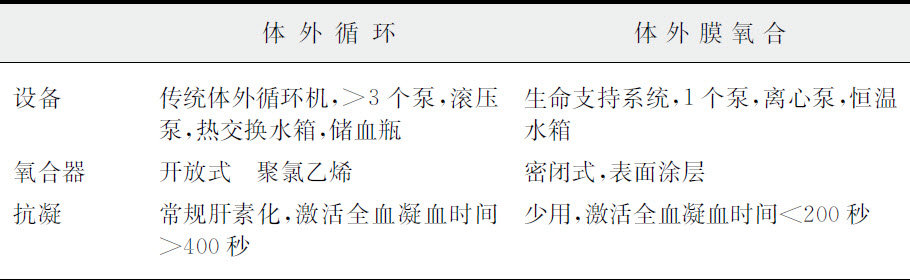
\includegraphics{./images/Image00281.jpg}
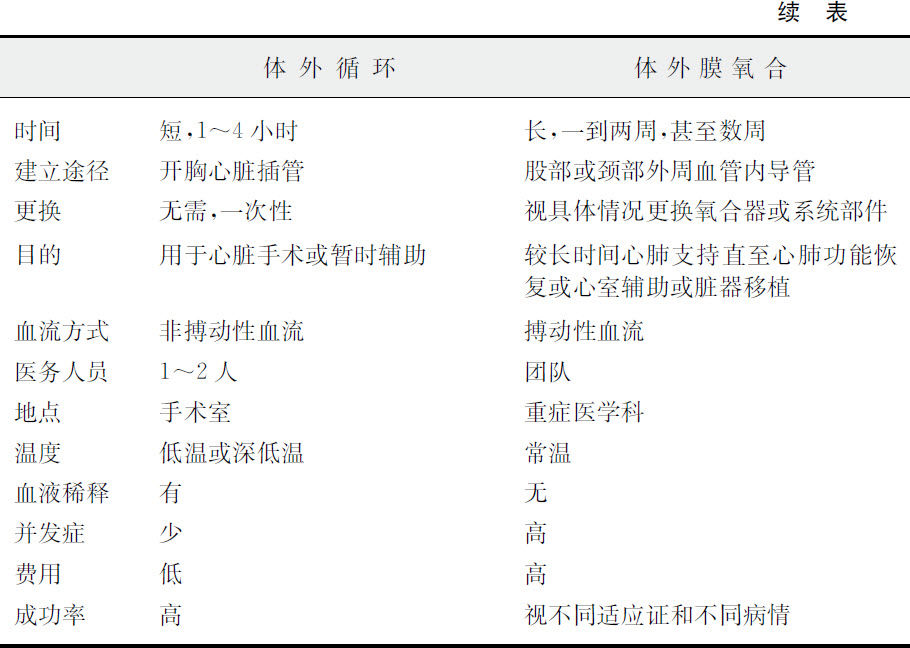
\includegraphics{./images/Image00282.jpg}
\end{table}




以上特点使体外膜氧合可以走出手术室成为生命支持技术。肝素涂层技术明显缩短激活全血凝血时间水平(120~180秒),显著减少出血并发症,尤其对有出血倾向的病人有重要意义。较低的激活全血凝血时间水平可在不加重原发病的基础上支持呼吸功能,为患者呼吸功能的恢复赢得时间。仅需要外周血管内置管、简便快速的操作使得体外膜氧合可在手术室外的条件下以极快的速度建立循环,从而使体外膜氧合可广泛应用于临床急救。

\subsubsection{体外膜氧合有哪几种转流方式?}

体外膜氧合基本转流方式主要有:V-V转流与V-A转流两种,另外还有V-A-V转流,A-A-A转流,A-V转流(无泵的二氧化碳清除)等。

(1)V-V转流 即将静脉血在体外经氧合器氧合、二氧化碳排出后通过另一静脉回输体内。通常选择股静脉引出静脉血,氧合后的血液经颈内静脉输入,也可根据病人情况选择双侧股静脉。V-V转流适合单纯呼吸功能受损,无循环功能障碍、无心脏停跳危险的病例。在体外膜氧合支持可下调呼吸机支持参数至氧浓度<60%、气道压<30cm
H\textsubscript{2}
O,仅仅给予小潮气量和维持肺膨胀的呼气末正压,从而避免为维持氧合而进行高条件呼吸支持治疗。需要强调的是,V-V转流是只可部分代替肺功能。

(2)V-A转流 即将静脉血引出经氧合器氧合并排出二氧化碳后回输入动脉。成人通常选择股动、静脉;新生儿及幼儿由于股动、静脉偏细而选择颈动、静脉;也可开胸手术行动、静脉置管。V-A转流是可同时支持心肺功能的连接方式,适用于心衰竭或心肺衰竭的病例。V-A转流方式时,未完全氧合的混合血流经过肺后灌注冠状动脉、右上肢和头部,与股动脉灌注氧合血流在主动脉弓水平混合,形成压力平衡界面,导致右上肢和头部血流由未完全氧合的血流供应。由于V-A转流体外膜氧合管路是与心肺并联的管路,可将80%回心血流引至氧合器,流经肺的血量减少,降低肺动脉压和心脏前负荷,但运转过程会增加心脏后负荷。此法缺点是股动脉低部位灌注使上半身的冠状动脉和脑组织得不到充分的灌注。有人将动脉导管延伸至主动脉根部以缓解这一难题,但这增加了血栓形成的危险,并有可能造成动脉机械性损伤。另外肺循环血流骤然减少,使肺的血液淤滞,增加了肺部炎症和血栓形成的危险性。目前认为在体外膜氧合治疗中维持一定的肺血流和肺动脉压力,有利于肺功能和结构的恢复。

(3)V-A-V转流 V-A转流方式时,未氧合的上腔静脉血流经过肺后灌注冠状动脉、右上肢和头部,在呼吸功能障碍的情况下,这部分静脉血得不到充分的氧合,因此导致右上肢和头部血流氧供减少。V-A转流时将膜肺后的氧合血分成两部分,一部分通过动脉回输,另一部分通过上腔静脉回输到右心,形成V-A-V的转流方式,增加经肺血流的氧合程度,达到改善右上肢和头部氧供的目的。

(4)A-V转流 A-V转流也被称为无泵的二氧化碳清除系统(extra corporeal
CO\textsubscript{2}
removal),是通过股动、静脉插管,依靠动静脉压力梯度,驱动血流流经氧合器,流量由动、静脉压力差和膜肺及管路的阻力决定,平均动脉压>70mmHg可保证血流量以清除二氧化碳,但是并不能完全支持氧合。A-V转流为搏动性血流,不需要泵的驱动,可降低血栓形成以及避免机械性血液损伤,但动、静脉分流对患者血流动力学和组织灌注会造成一定影响。

(5)A-A-A转流 当心脏完全停止跳动,V-A模式下易产生部分血液滞留,从而导致血栓形成、产生不可逆损害。此时,需要开胸手术置管,将血液分别从左、右心房引出经氧合器氧合并排出二氧化碳后泵入动脉。该转流方式可防止心肺内血栓形成并防止肺水肿发生。如果超声诊断下心脏完全停止跳动>3小时则应立即开胸手术置管转换成A-A-A模式。

\subsubsection{V-A和V-V转流体外膜氧合有何不同?}

V-V和V-A转流体外膜氧合明显不同,各自具有优缺点(表\ref{tab24-2})。

\begin{table}[htbp]
\centering
\caption{V-A和V-V转流体外膜氧合的异同项}
\label{tab24-2}
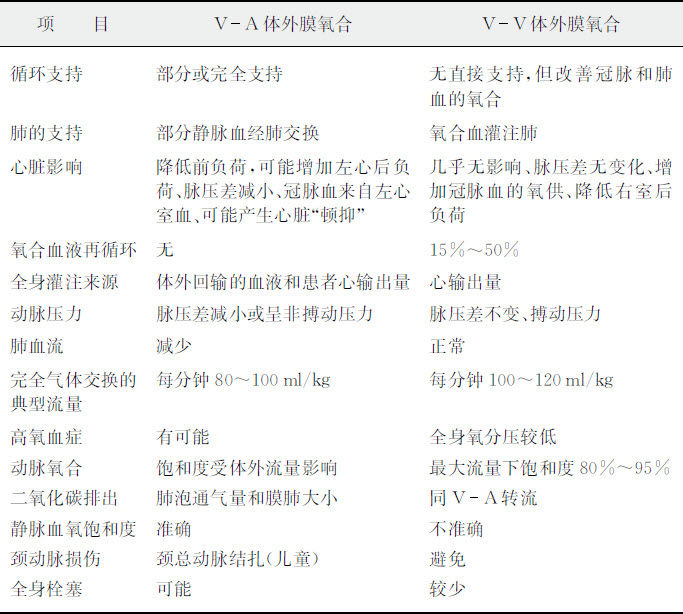
\includegraphics{./images/Image00283.jpg}
\end{table}

与V-A相比,V-V转流体外膜氧合可避免肺血流减少引起的缺血性肺损伤;由于直接提供氧合血进入肺循环,有利于减少肺的炎性反应;血液经静脉回流,血由心脏射血维持组织灌注,因而保留了生理性的搏动灌注,有利于降低血管阻力和心脏后负荷,改善器官灌注,尤其优于V-A模式下脑灌注。

\subsubsection{如何选择体外膜氧合的转流方式?}

体外膜氧合正确的转流方式选择利于原发病的治疗和提高治疗成功率。临床治疗中要参照病因、病情,根据患者具体情况灵活选择。总体来说V-V转流为肺功能替代的转流方式,V-A转流为心肺联合替代的转流方式。呼吸衰竭选用V-V转流方法;心脏衰竭及心肺衰竭选V-A;长时间心跳停止选择A-A-A模式。另外,治疗过程中,随病情的变化,还可能需要变化转流方式,例如心肺衰竭选择V-A转流方法,经过治疗心功能恢复而肺功能尚未恢复,仍需要替代治疗,此时需转为V-V模式继续支持。

\subsection{体外膜氧合的适应证和禁忌证}

\subsubsection{体外膜氧合有哪些适应证?}

体外膜氧合主要用于急性的、对常规治疗无反应、预计2~4周内能恢复或改善的或有器官移植等相应后续治疗措施的可逆性心肺衰竭的治疗,为原发病的进一步治疗和病情恢复争取时间。

(1)急性严重呼吸功能衰竭 急性严重呼吸功能衰竭是体外膜氧合支持成功率最高的疾病类型。主要用于常规治疗无效的重症ARDS、急性肺栓塞、重症哮喘等疾病,尤其是新生儿急性呼吸衰竭有较高的成功率。治疗原则是尽快建立稳定的生命支持,缩短器官缺氧时间。通常需要较长支持时间,一般选择V-V转流,氧合器首选膜式氧合器。对于肺挫伤首选V-A转流方法,有利于减少肺血流,同时可应对可能发生的肺出血。呼吸机治疗的参数可在体外膜氧合支持下调至肺休息的安全范围内。

(2)急性严重心功能衰竭 体外膜氧合治疗常用于各种原因导致的对常规治疗无反应的严重心源性休克,如重症爆发性心肌炎、心脏外科术前支持或手术后、急性心肌梗死等,还可以用于其他原因导致的严重心功能抑制状态下的急性循环功能衰竭,如药物过量。严重的心脏衰竭不但会减少组织器官血供,更严重的是随时会有心跳骤停的可能。体外膜氧合可改善心脏本身及其他器官的氧合血供,降低心跳骤停的风险。在体外膜氧合实施同时进行主动脉内球囊反搏治疗,有利于降低心脏后负荷、改善冠脉循环、促进心功能恢复。

(3)各种原因引起的心跳呼吸骤停 心跳呼吸骤停在传统急救的同时实施V-A体外膜氧合治疗有利于在最短的时间内建立呼吸循环,保护心脑等重要脏器灌注;防止反复出现心跳呼吸骤停;为心跳呼吸骤停病因的诊断和治疗赢得时间。经过训练的团队可以将体外膜氧合的启动时间控制在8~15分钟。在有效的心肺复苏支持下,团队密切合作尽快启动体外膜氧合治疗,可以缩短组织器官缺血缺氧的时间。实施体外膜氧合支持下寻找原发症并积极治疗。无原发病的患者可在去除刺激因素后迅速脱离体外膜氧合系统,如电击、高血钾等导致的心跳呼吸骤停。某些原发病经过支持可以逐渐恢复,待恢复后可脱离体外膜氧合系统,例如重症爆发性心肌炎。若有严重的原发病且非自限性,如不治疗心功能难以恢复,应迅速进一步治疗,如急性心肌梗死,需在体外膜氧合支持下多科协作治疗,尽快实施冠状动脉搭桥手术或冠状动脉支架植入术是可迅速恢复心功能的。由于脑功能的丧失恢复困难,因此,确定脑功能丧失是终止体外膜氧合的重要指征之一。

(4)器官移植 对于一些心肺功能没有恢复可能的病例,仍能通过日益发展强大的移植技术来脱离体外膜氧合达到康复。这就使一些被认为是禁忌证的疾患仍可延伸使用体外膜氧合技术,并与移植技术结合,形成一个理想的救治过程,甚至促进了移植技术的发展。目前已有一些医疗中心在做这方面的探索,并取得了一定成绩,而这一切工作的基础就是其他器官的保护,避免多个器官损害是成功的关键。

\subsubsection{体外膜氧合的禁忌证是什么?}

体外膜氧合的禁忌证包括绝对和相对禁忌证。

(1)相对禁忌证:①机械通气>7天;②无法建立合适的血管通路;③肝素抗凝禁忌;④高龄患者(年龄>70岁);⑤转移性恶性肿瘤;⑥进展性肺纤维化;⑦严重创伤和颅脑出血手术后早期;⑧无法解决的外科问题。

(2)绝对禁忌证:①无法进行抗凝治疗;②不可逆转的脑损害;③其他不可逆状态,如疾病终末期。

\subsection{体外膜氧合的临床实施}

\subsubsection{体外膜氧合治疗前需要做哪些准备?}

体外膜氧合有时需要紧急操作,争分夺秒,如心跳呼吸骤停患者。有些病例虽没有那么紧急,但也是需要尽快启动,避免缺血缺氧导致的器官功能损害加重。通常应将体外膜氧合设备放置在可移动的转运车上,便于转运。体外膜氧合前需要准备的设备、器材和药品包括离心泵、阻断钳、空氧混合器及气源、变温水箱、ACT监测仪和检测管、血气仪、连续血氧饱和度监测仪及连接玻管、转运车等、PLS套包及其支架、动(静)脉血管内导管,体外膜氧合导管插管套包、预充液、肝素等。

\subsubsection{怎样选择合适的体外膜氧合血管内导管?}

选择合适的体外膜氧合血管内导管是建立体外膜氧合血管内通路的前提,也是提供合适的血流量、避免血管并发症的基本保障。体外膜氧合流量和避免血管并发症的发生是选择体外膜氧合导管的主要依据。在体外膜氧合系统中,在容量足够的情况下,流量取决于插管的管径和阻力。插管的阻力与插管的长度成正比、与管径的4次方成反比。因此选择静脉引流管的原则为内径应尽可能大、长度尽量短。选择管壁薄而坚固、带有钢丝缠绕设计的插管不容易发生折曲和挤压变形。

以V-A辅助为例,正常心排量3.0~3.5L/(min·m\textsuperscript{2}
),体外膜氧合治疗流量至少需能达到2.5~3.0L/(min·m\textsuperscript{2}
)。而V-V辅助则要求的流量要大一些,为3.0~3.5L/(min·m\textsuperscript{2}
)。股动脉插管时,应尽可能选择较细的导管避免发生远端肢体缺血。如静脉引血管流量不足,可在另一侧股静脉或是头侧颈内静脉插管附加第二根引流管增加引流量。

另外,由于各个厂家体外膜氧合导管工艺和材料存在差异,导管厂家都会提供流速压力阶差表。以Maquet的导管为例,100kg体重患者,动、静脉各有100mmHg压力阶差的情况下,要选择动脉PAL
1915、静脉PVL
2155的插管,即19F动脉和21F静脉导管,可实现5L/分的流量。这样在5L/分流量的情况下需要的驱动力压为100mmHg+100mmHg+50mmHg=250mmHg。离心泵所能提供的驱动力为600mmHg。但太高的转速下血细胞破坏也比较严重,要尽量避免。通常,250~300mmHg的压差是可以接受的。

为方便日常工作,可根据患者体重初步选择导管,可参考表\ref{tab24-3}~表\ref{tab24-4}。

\begin{table}[htbp]
\centering
\caption{V-A转流体外膜氧合导管管径大小选择}
\label{tab24-3}
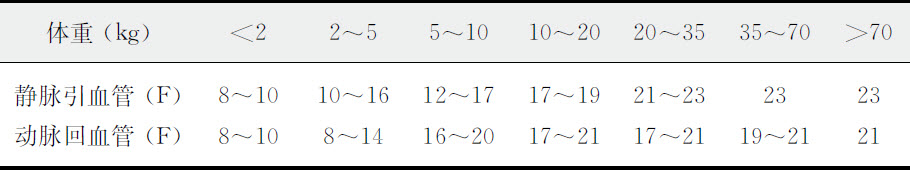
\includegraphics{./images/Image00284.jpg}
\end{table}

\begin{table}[htbp]
\centering
\caption{V-V转流体外膜氧合导管管径大小选择}
\label{tab24-4}
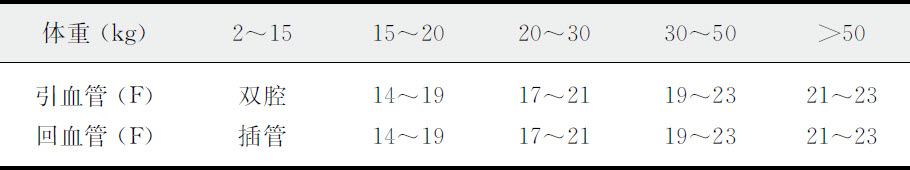
\includegraphics{./images/Image00285.jpg}
\end{table}

\subsubsection{如何建立体外膜氧合血管通路?}

建立并维持良好的血流进出通路是体外膜氧合支持的关键。正确、合理的插管方式以及良好的置管技术是血流出入通畅的保证。目前常规体外膜氧合血管内导管置入方式包括穿刺法和切开法两种。

(1)穿刺法 目前有体外膜氧合血管内导管穿刺置管套包供临床使用,采用Seldinger法进行置管。按常规消毒、铺巾、局部麻醉后,超声引导下穿刺目标血管,通过穿刺针芯将导引钢丝置入血管内,退出穿刺针。根据导管直径穿刺点切开皮肤和皮下组织,沿导引钢丝扩张血管,注意避免血肿和出血。带有内芯的体外膜氧合导管沿导引钢丝置入,根据不同血管和穿刺部位置入合适的位置。

床边操作时,置管前应先初步测量需置入导管的深度(如股动脉一般为股动脉穿刺点至髂总动脉)。操作结束后X线检查或超声检查确定导管尖端位置。若在床边X线或超声指导下操作,可直接放置到合适位置。

在开始体外膜氧合运行时,需要密切关注氧合器前后的血流颜色改变,氧合器之前为暗黑色的未氧合血,氧合器之后为鲜红色的氧合血,如在体外膜氧合运行过程中出现颜色均变为暗黑色或鲜红色,须注意导管位置是否合适。

操作后注意牢固固定导管,以防滑出,局部可用无菌敷料覆盖防治局部感染,面积应覆盖穿刺点周围10cm以上的范围。如无明显渗血可换用无菌手术贴膜覆盖。

(2)切开法 手术分离出股动、静脉或颈部血管,直视下插入导管。适用于穿刺困难的病例如休克、股动脉硬化者、股动脉触摸困难者或体外循环术中。由于需手术植入,操作费时,出血和感染的机会多,且停用后还要行动、静脉修补术,现在多被穿刺法取代,只在穿刺法失败或无法进行穿刺才考虑使用。

\subsubsection{如何进行体外膜氧合管路连接和预充?}

在建立体外膜氧合循环之前,必须建立血管内通路和准备好管路及预充等准备工作,一般由多名医师配合同时进行,便于快速建立体外膜氧合循环。如下为使用离心泵建立体外膜氧合之前连接管路和预充的基本步骤。

(1)准备预充液,管路预充液一般选用平衡盐液2000ml加肝素UFH(预充液内肝素5mg/500ml)配置而成。也可根据患者情况加入白蛋白、血浆、红细胞(多用于婴幼儿)。根据患者循环状态决定预充液是否进入病人体内;

(2)检查管路外包装、有效期,套包条形码粘贴在操作记录单上;

(3)连接静脉引流管与离心泵头口,连接紧密,扎带固定;

(4)连接两根预充管,将两根预充管中间管路用阻断钳阻断;

(5)将靠近离心泵头静脉端预充管(标为1号管)针头插入预充袋内,利用重力排气超过离心泵头,排气钳夹预充管(标为1号钳);

(6)另一预充管(标为2号管)针头插入预充液袋内,备排气,钳夹预充管(标为2号钳);

(7)均匀涂层导电糊后将离心泵头装入离心泵,离心泵转速逐渐调至2000RPM,松1号钳,打开2号管三通,预充氧合器与管道,充分排气,管道内无明显气体后将三通旋向预充袋方向;

(8)氧合器内无明显气体,氧合器预充完全,1号和2号钳钳夹阻断两根预充管,关闭预充管三通,松两根预充管中间的阻断钳,旋紧氧合器上黄色肝素帽,再次确认管路内预充情况,如有气体再次预充;

(9)预充结束,管路自循环备用,去除1号和2号管;

(10)理顺整个循环管路,并固定于适当位置,避免管道弯折;

(11)连接空氧混合气管道(气源→空氧混合器→氧合器),设定吸入氧浓度和气体流量;

(12)连接变温水箱,设置适宜水温,并进行水循环,

(13)待台上动、静脉导管置入确认后,打开台上管包装,将管路递给台上操作医师;

(14)再次确认管路内无气体,管路通畅无误,连接管路准备运行体外膜氧合。

\subsubsection{体外膜氧合过程中的抗凝选择和监测内容有哪些?}

体外膜氧合的抗凝是维持运转和系统使用时间的重要关键因素。由于目前体外膜氧合多采用肝素涂层技术,抗凝并不像体外循环要求完全肝素化。通常采用普通肝素抗凝,负荷量5~50U/kg之后给予小剂量持续静脉每小时5~20U/kg泵入,定时监测ACT,维持在160~200秒。无活动出血维持ACT在160~200秒;有活动出血者维持在130~160秒;辅助流量减低时需维持ACT在高限水平;高流量辅助、脏器出血或胸腔引流进行性增多时,ACT可维持在低限水平。

对没有出血危险的病例,常规监测参数包括血小板计数,维持在10×10\textsuperscript{9}
/L以上、凝血酶原时间正常范围、纤维蛋白原>100mg/ml。另外还需要注意特殊病人的抗凝需要密切监测,如肝素耐药患者、凝血因子缺乏患者、孕产妇往往处于高凝状态等。输注血小板、血浆等促凝物质时应从氧合器后加压输注,避免血小板和血浆等由外周输注经静脉引流直接进入氧合器,激活和导致氧合器凝血;在加压输注过程中严格无菌操作,避免致命性的血源性感染。

\subsubsection{如何进行体外膜氧合运行初始设置和参数调整?}

预充结束和体外膜氧合导管置管成功后,将体外膜氧合导管和预充的管路连接紧密,注意防止气泡进入,如管路连接处有少量进气,可在管路连接处三通连接注射器,打开导管阻断钳,抽出气泡。

根据转流方式和患者病情进行初始设置,包括初始泵速、气体流量和吸入氧浓度,再次确认设置无误后开放体外膜氧合管道通路,开始运行体外膜氧合。

V-A转流体外膜氧合的初始设定血流速一般为1.5~2.0L/分,或体外循环不能脱机患者根据体外循环过程中的设置估计大致辅助流量,吸入氧浓度设置为0.5~0.6,气体流速根据血流速设定,气体流速与血流速比例设定为1∶1。

V-V转流体外膜氧合的初始设定血流速一般为2.0~4.0L/分,吸入氧浓度设置为0.6~1.0,气体流速根据血流速设定,气体流速与血流速比例设定为1∶1~2∶1。

初始设定后根据患者病情需要调节参数设置,维持氧饱和度在92%以上、动脉氧分压>80mmHg、动脉血二氧化碳分压<50mmHg、平均动脉压>65mmHg、氧输送/氧消耗>4∶1、维持患者生命体征稳定。每日根据体外膜氧合特护单和检查单进行离心泵、膜肺、管路和运行情况的监测和记录。

\subsubsection{影响体外膜氧合流量的因素是什么?}

影响体外膜氧合流量的因素主要包括患者自身因素、血管内导管、连接管路、氧合器和动力泵多方面因素。

体外膜氧合流量下降伴静脉管路明显抖动可见于患者容量不足、咳嗽或烦躁、静脉引流管位置不当、内径过细或堵塞扭曲、连接管路打折扭曲或受压等导致流量下降。

体外膜氧合流量下降而静脉管路不抖多为动脉管路和膜肺出现问题,常见的包括动脉管路位置不当、堵塞或扭曲、氧合器凝血等。

\subsubsection{什么是V-V转流的再循环和再循环血流分数?}

正确理解再循环的概念是V-V辅助成功与否,并能够准确评价V-V转流模式下血气结果的关键。部分回流的氧合血可能直接进入静脉引流管被引流再次进行氧合而没有进入患者的体循环,这部分血流定义为再循环血流。

再循环血流分数(R)的计算公式为:

\[R=\frac{S_{pre}O_x-SVO_2}{S_{post}O_x-SVO_2}\]

SpreOx为进入氧合器前的血氧饱和度,SpostOx为出氧合器后的血氧饱和度,S\textsubscript{V}
O\textsubscript{2}
为患者的实际混合静脉血氧饱和度。如果用氧含量替代氧饱和度,这个公式结果将更加准确,但对于临床应用来说这个差别很小。如果回流到氧合器氧饱和度较高的血量增加,SpreOx也会相应增加接近SpostOx,R值随之增加。

\subsubsection{V-V转流影响再循环的因素是什么?}

了解影响再循环的因素远比计算再循环的量更为重要。影响再循环的四个主要因素是体外膜氧合流量、静脉插管位置、心输出量和右心房血容量。

流量对再循环的影响显而易见。当流量增加时,右心房引流到体外膜氧合环路的血量随之增加,这样来自体外膜氧合的氧合血很有可能被再次引流到环路中。再循环流量分数的增加与泵流量呈线性关系。患者的氧供随着流量的增加而增加,但当超过最佳流量和最小再循环后,氧供即随流量的增加而减少。这是由于再循环的比例限制了患者氧供的总量导致的。流量可以通过下面的公式来表示:

有效泵流量=泵的总流量-(泵的总流量×再循环流量分数)

有时再循环甚至会高达100%,有效血流量只有零。理想的流量是在最低的转速下提供最高的有效血流量,产生最小程度的溶血。

V-V转流体外膜氧合的最佳流量并不是固定的,因为还有其他3个因素影响:插管位置、心输出量和右心房容量。如果引流管和供血管的尖端直接相对,再循环就会很高。使用双腔插管时,如果插管位置位于上腔静脉或位于下腔静脉,回输到体内的血会限制在血管腔范围内,在进入右心房之前就被引流入体外膜氧合环路。这种现象解释了为什么插管位置变化时患者的动脉氧饱和度会意想不到的快速降低。肺膨胀程度的变化、颈部缝合固定部位水肿、患者体位的变化和患者的移动都会改变插管的位置。

心输出量也会影响再循环。如果进入右心房的氧合血大部分进入右室,随后进入左心和体循环,那么只有很少的氧合血再次进入氧合器。相反,由于没有前向血流,回到右心房的氧合血全部再次引流入氧合器。通过增加心输出量可以减少再循环而增加氧合总量。同样原因,右心房容量也影响再循环的比例。如果右心房未氧合血容量减少,氧合血会更趋向于再回到氧合器内。但如果右心房氧合血在正常容量的右心房被大量的非氧合血稀释的话就会减少再循环的程度。因此,补充血容量能快速减少再循环的程度,更有效地增加氧供。但立即减少再循环的益处需要与增加血管外肺水含量的弊端相权衡。

由于V-V转流体外膜氧合不直接提供循环辅助,所以要达到与V-A模式相同的氧供水平会比较困难。但如果最大程度减少再循环并维持心脏支持的话,氧供水平可以接近V-A模式。血红蛋白达到15g/L、再循环较低、静脉引流达到每分钟120~140ml/kg的情况下,可以达到最佳氧合状态。

如果在不增加再循环的部位增加一根引流管(如股静脉加颈内静脉头侧插管至壶腹水平),可以明显增加氧供。氧供的增加来自再循环的减少。头侧的第二根静脉还可以起到降低颅内静脉压的作用。由于来自颈内静脉壶腹部的混合静脉血氧饱和度较低,所以可以从氧合器得到更多的氧。尽管理论上很好,但体外循环生命支持组织的数据没有证明V-V转流体外膜氧合中常规颈内静脉插管引流会改善新生儿急性呼吸衰竭的预后。

\subsubsection{体外膜氧合期间如何设置呼吸机参数?}

体外膜氧合患者临床上通常都存在不同程度的肺病变和呼吸功能不全,从轻度的心源性肺水肿(当体外膜氧合用于心脏支持时)到严重的完全的肺失功能(当体外膜氧合用于呼吸支持时)。在这种情况下,一旦之前存在的高气道压力降低,原本被过高的膨胀压维持开放的小气道和肺泡常常塌陷,导致X线胸片上呈现充血和实变征象,以及自体肺无气体交换征象。这在V-V和V-A模式下都可能发生。为了减少全肺实变,平均气道压应维持在10~20cm
H\textsubscript{2} O。

V-A转流模式下,由于大量静脉回心血液被引流至体外循环,肺血明显减少,肺内可出现广泛的通气血流不匹配,最常见是与肺毛细血管床血流减少相比,即便是低水平通气也产生相对通气过度。这可能造成大量死腔通气,表现为低呼气末二氧化碳。如果这种通气血流比例失调通过降低机械通气参数如降低通气压力来治疗,可能最终造成肺泡塌陷。所以在V-A转流模式下,最好维持呼气末正压在10~15cm
H\textsubscript{2} O,限制吸气相气道平台压≤30cm H\textsubscript{2}
O,形成小潮气量低频呼吸。即使在这种设置下,仍有可能造成二氧化碳过度排出,可以通过同时在体外循环系统通气中加入一定二氧化碳气体来解决。

V-V转流体外膜氧合治疗严重肺功能不全期间的目的是尽可能挽救肺泡功能,并避免进一步的呼吸机肺损伤。这可通过维持平均气道压在10~20cm
H\textsubscript{2} O,限制气道峰压<30cm H\textsubscript{2}
O,呼气末正压设置为8~10cm H\textsubscript{2}
O,潮气量设置为4(3~6)ml/kg(预计体重),并维持吸入氧浓度<50%来实现。同时可以采用的治疗严重肺损伤的方法包括俯卧位通气、体位引流、维持患者偏“干”、充分营养和必要时进行纤维支气管镜检查。

\subsubsection{体外膜氧合期间如何进行镇静镇痛治疗?}

患者在接受体外膜氧合之前由于缺氧、酸中毒和低灌注可能导致脑损伤,所以需要密切监测神经系统功能。由于体外膜氧合建立时,患者往往处于病危情急阶段,生命体征不稳定,需要较多的有创性操作,大多数患者在体外膜氧合前处于深度镇痛和镇静状态,开始体外膜氧合时无法进行神经系统评估,所以使患者从镇静和麻痹状态中苏醒是第一步。

体外膜氧合运行过程中,患者生命体征在体外膜氧合支持下明显好转,可根据患者情况适当减轻镇静镇痛深度,维持昼夜节律,在评估患者神经系统和镇静深度的情况下,保留患者自主咳嗽等保护反射,减少肺炎等过度镇静导致的并发症。但在减轻镇静的过程中注意保护导管安全,适当约束,避免出现位置不当甚至出现严重后果。

在体外膜氧合支持后期患者病情进一步好转,可进一步减轻镇静,但需维持患者昼夜节律,为撤机拔管做准备。

\subsubsection{体外膜氧合期间如何常规进行监测?}

体外膜氧合治疗前需要全面了解患者凝血功能和状态、电解质、肝肾功能、呼吸功能等。体外膜氧合建立后,X线摄片或B超确认并调整导管位置,测量血管内导管外露长度并每日进行测量。肝素抗凝患者上机后每3~4小时监测激活全血凝血时间,随监测调整肝素用量,输注血小板、血浆或大量蛋白后会导致患者凝血功能改变,需要输注后30分钟再次测定激活全血凝血时间;如有血小板下降或部分激活的凝血活酶时间明显延长等出血倾向,将激活全血凝血时间下调至160秒左右。定期复查血常规、白蛋白水平、凝血功能、动静脉血气分析;定时监测体外膜氧合血流量、血压、管路搏动、肢端缺血情况、体温、镇静深度。以上定时检查和评估项目可作为体外膜氧合医疗护理常规建立表格进行记录。

\subsubsection{体外膜氧合运行过程中相关注意事项和处理内容有哪些?}

体外膜氧合的建立和运行是一个系统工程,需要训练有素的团队的精诚合作,保证体外膜氧合的顺利进行,避免并发症发生。在体外膜氧合运行过程中,有很多需要注意的问题和体外膜氧合相关的特殊处理。

(1)导管管路相关注意事项 ①体外膜氧合插管处无菌贴膜覆盖(覆盖穿刺点边缘超过10cm以上,无明显渗血,2~3天更换一次);②避免管路扭曲和成角;③管路缝扎固定后再绷带捆扎,分别固定于腿部或头部,保证引流和回血通畅,防止滑脱、翻身或活动时脱出或位置变动(翻身时专人固定引血管和回血管),检查并记录外露钢丝管长度。

(2)离心泵相关注意事项(MAQUET离心泵为例) ①离心泵报警显示“SIG”,提示离心泵超声探头导电胶干燥或不足导致流速探测故障,需停泵更换导电胶,步骤如下:夹闭管路动静脉端管路阻断血流;停止离心泵(转速调为0转);打开取出离心泵头;清水纱布擦洗玻管;再次均匀涂擦导电胶;安装离心泵泵头;设定泵转速;打开动静脉端阻断钳运行体外膜氧合;②离心泵失稳,剧烈晃动或撞击离心泵可能使离心泵头与泵座磁场失去耦合,导致离心泵失稳,离心泵泵头处可听见明显杂音,需要立即通知医生,钳夹动静脉端,停泵取下离心泵头再次安装恢复耦合后恢复正常运行;③密切关注体外膜氧合流量变化,在短时间内相同转速下血流速较基础降低0.5L/分,立即通知医生,首先关注管道是否打折扭曲,其次观察离心泵泵头或膜肺是否有凝血发生。

(3)体外膜氧合管理相关注意事项 如进出氧合器管路内血颜色变一致,颜色均变深考虑膜肺氧合不全,可能为供气管脱落、氧合器血栓、气体流速和血流速不匹配(V/Q失调)等所致;颜色均变鲜考虑V-V转流体外膜氧合时引血和回血端插管开口太近(再循环率增加);管路进气、漏血或血栓,立即以阻断钳钳夹动静脉插管处,阻止气体或血栓进入患者体内并立即通知医生,立即重新预充或更换套包;维持血红蛋白在10~13g/L,或血细胞比容在35%以上,增加氧输送;如患者尿色明显加深,考虑血液破坏导致溶血,查尿游离血红蛋白,也可尿液离心3000转/分后观察上清液颜色,如色深考虑溶血;如发生停电或离心泵故障,立即取下离心泵泵头,用备用手摇泵运转离心泵。

(4)抗凝和凝血监测相关注意事项 密切关注患者出血倾向,尽可能减少不必要的血管穿刺,气道吸引时注意有无气道出血,降低吸引负压;维持血小板在100×10\textsuperscript{9}
/L以上,低于50×10\textsuperscript{9}
/L必须及时输注血小板,输注血小板时,应在膜肺后回血端三通注射器推注,防止血小板静脉内输注后立即进入膜肺加重血小板膜肺内的消耗,导致膜肺凝血;常规应用肢体加压装置,防止下肢静脉(尤其是体外膜氧合插管处)血栓形成。

(5)感染相关注意事项 严格无菌操作,所有血管通路和管路操作均需清洁手后无菌下进行;维持鼻咽温35.5~36.6℃,防止寒战和高热,预防低温,同时警惕感染引起持续低热。

(6)营养支持相关注意事项 尽可能给予肠内营养,避免输注脂肪乳,如必须输注尽量减慢脂肪乳输注速度(脂肪乳自由基破坏膜肺中空纤维膜,影响膜肺氧合),尽可能不使用异丙酚镇静。

\subsection{体外膜氧合的撤离}

\subsubsection{体外膜氧合撤离筛查标准是什么?}

体外膜氧合是患者心肺功能衰竭时临时支持措施,其终极目标是自身心肺功能恢复后尽快撤除,或通过其他长期支持治疗措施的实施,在患者病情改善时,应尽快撤除体外膜氧合。判断患者病情是否适合进入撤除体外膜氧合的程序,需要对患者病情进行判断,也就是需要进行体外膜氧合撤离的筛查,以下是根据文献和临床列出的初步筛查标准:

(1)原发疾病改善或得到控制;

(2)肺部X线影像好转,氧合良好;

(3)体外膜氧合血流速减低至1.5~2L/分;

(4)最低剂量的正性肌力药物,肾上腺素≤0.04μg/(kg·分);

(5)心脏指数>2.0L/分·m\textsuperscript{2} ;

(6)肺动脉嵌顿压和(或)中心静脉压<16mmHg;

(7)动静脉血气分析结果良好,无组织灌注不足表现。

\subsubsection{如何评估患者能否撤离体外膜氧合?}

进行每日筛查,如达到撤离体外膜氧合的筛查标准,根据患者病情和采用的转流模式开始体外膜氧合自主循环试验(spontaneous
circulation trial)和自主呼吸试验(spontaneous respiratory trial)。

循环功能评估:当患者心功能好转,体外膜氧合循环辅助流量≤1L/分时进行自主循环试验。将血流速降为1L/分,或阻断动静脉插管通路,开放体外膜氧合桥,流量减至0.5L/分,观察6小时,血压、心率较基础值变化大于20%则继续行体外膜氧合支持,如呼吸循环各项指标变化低于20%,无明显组织灌注不足表现,可考虑撤离心脏辅助。

呼吸功能评估:进行自主呼吸试验(体外膜氧合血流速不变,关闭膜肺气体进气口和出气口,使膜肺完全停止氧合),吸入氧浓度≤60%;呼气末正压≤5cm
H\textsubscript{2}
O;观察10分钟,如动脉血氧饱和度>92%,动脉血二氧化碳分压<50mmHg;静态肺顺应性≥0.5ml/(cm·kg),混合静脉血氧饱和度维持在70%以上,心率、血压、氧合波动小于20%,继续观察6~24小时,心率、血压、氧合波动小于20%,血气分析未有明显恶化,组织灌注良好,可考虑撤离V-V转流体外膜氧合。

\subsubsection{体外膜氧合撤离流程是怎么样的?}

患者心肺功能恢复,进行每日筛查,通过撤离体外膜氧合评估的自主循环试验和(或)自主呼吸试验,结合患者病情,即可考虑体外膜氧合撤离。将体外循环的血液经自体血回输装置回输患者体内或弃去,动脉插管需行动脉缝合术,防止远端组织缺血,股静脉需要外科修补,颈内静脉插管可直接拔管,拔管后需要按压1小时以上,并予以鱼精蛋白中和肝素,使全血激活凝血时间恢复正常水平,注意穿刺点局部有无出血。详见图\ref{fig24-1}。

\begin{figure}[!htbp]
 \centering
 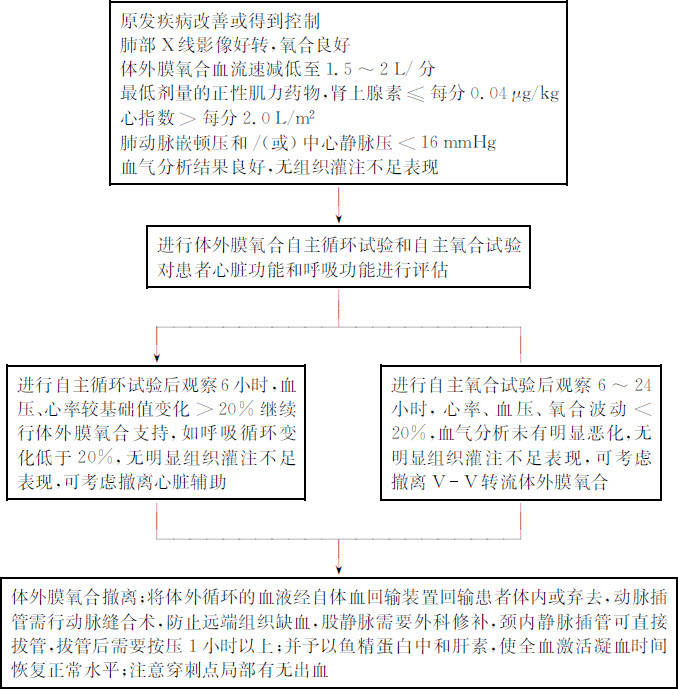
\includegraphics{./images/Image00287.jpg}
 \captionsetup{justification=centering}
 \caption{体外膜氧合的撤离流程}
 \label{fig24-1}
  \end{figure} 

\subsection{体外膜氧合的并发症及防治}

\subsubsection{体外膜氧合有哪些并发症?}

进行体外膜氧合治疗的患者病情危重,机械辅助生命支持过程中并发症难以完全避免。缩短体外膜氧合支持时间,是防治体外膜氧合并发症的最好方法。出现并发症不一定可怕,最可怕的是在错误的时间由没有经验的人做出了错误的医疗行为,导致不可挽救的临床后果,甚至直接威胁患者生命。

体外膜氧合常见并发症包括体外膜氧合相关机械并发症和患者相关并发症两大类,详见表\ref{tab24-5}。

\begin{table}[htbp]
\centering
\caption{体外膜氧合常见并发症}
\label{tab24-5}
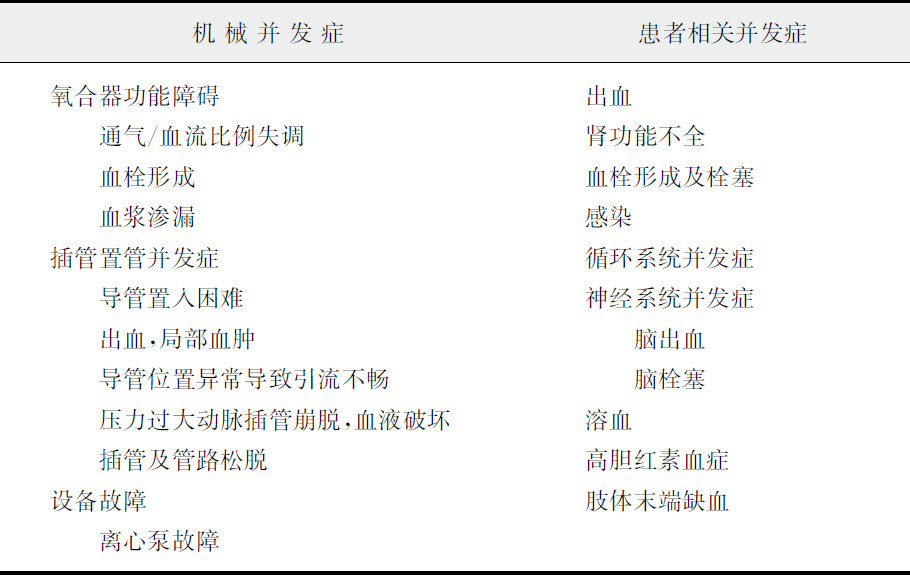
\includegraphics{./images/Image00288.jpg}
\end{table}

\subsubsection{体外膜氧合常见机械并发症的危害和原因是什么?如何防控?}

体外膜氧合常见机械并发症包括氧合器功能障碍、血管内导管相关并发症和设备故障。

(1)氧合器功能障碍 氧合器功能障碍是体外膜氧合常见的并发症,体外循环生命支持组织报告氧合器功能障碍发生率新生儿为6%、儿童约13.7%、成人约18%。主要原因有静水压升高超过膜的抗渗透能力导致血浆渗漏,通气/血流比例失调导致氧合或二氧化碳清除障碍,膜肺内血栓形成导致跨膜肺阻力升高,离心泵相同转速下的血流量明显下降等。预防氧合器功能障碍首先选择合适的氧合器;合理掌握氧合器使用安全时限;每日定时“吹”氧合器(高流速通气1分钟);避免使用破坏氧合器膜的药物进入循环;并密切监测氧合器功能,可以采用氧合器定时检查单方式对氧合器功能相关指标定期检查,以判断氧合器功能状态和发生障碍的原因。氧合器定期检查单内容包括氧合器气体流量是否与血流量匹配,氧合器血流量是否在氧合器性能范围内,气体管道连接是否正确,氧合器气体出口是否开放,氧合器气体出口内积液是否清亮,氧合器顶端是否有气泡,氧合器前后压力差,目视氧合器内有无血栓形成。

(2)血管内导管相关并发症 血管内导管并发症总发生率婴儿约11.2%,小儿约13.6%,成人约10.8%。常见并发症包括血管损伤;插管位置异常导致引流不畅或灌注压力增大导致血液破坏,甚至插管崩脱;导管与管路连接处松脱导致大量出血。

预防血管内导管并发症需要定期检查血管导管是否缝扎固定;导管穿刺点有无活动性出血或渗血;管道内有无凝块;插管是否固定在患者身体上/床边/其他固定器;插管口径选择是否正确;插管位置在X线片和超声下位置是否正确,有无移位;患者肢体是否约束。

(3)血栓形成 血栓事件发生率婴儿大约18.3%,小儿6.9%,成人约9.5%。血栓形成可导致体外膜氧合系统失去功能,凝血因子大量消耗,甚至患者动脉栓塞/肺栓塞。

预防和控制血栓形成事件的发生应尽可能选择肝素涂层管道;避免体外膜氧合管路有死角和扭曲;体外膜氧合运行期间需要完善常规抗凝,监测激活全血凝血时间维持在180~220秒左右;输入红细胞、血小板等血液成分时加大抗凝药物剂量;根据肝素代谢调整抗凝药物剂量(根据经验和激活全血凝血时间变化趋势,注意时间提前量);控制出血时常留警惕之心,避免过度止血导致血栓;维持体外膜氧合循环足够血流量,如有局部血栓形成,可考虑更换局部或整套管路。

(4)空气栓塞 由于静脉端为负压,插管或管道接口破裂或密封不良可以导致静脉端进气,导致氧合器功能障碍。如静脉端气体到动脉;操作失误导致膜肺内气相压力高于血液相;氧合器膜破裂,血液凝固于出气口,使气相压力逐渐增高均可导致动脉端也就是回输端进气,导致患者出现气体栓塞。

预防和避免出现气体栓塞首先要保证插管、管道和接头连接的完整性;避免静脉段过度负压;及时驱除进入体外膜氧合系统的气体,微量或少量气体可被离心泵和氧合器捕捉,中量、大量进气需要停机,重新排气;在体外膜氧合运行过程中需密切观察,特别是出现血浆渗透时,避免出气口被血凝块堵塞,导致气相压力升高导致气栓。

大量进气应紧急处理,处理措施包括如下几个方面。发现体外膜氧合系统内进气立即夹动静脉管路并立即停机;同时提高其他辅助生命支持手段如调节呼吸机支持条件,调整血管活性药物剂量等维持患者生命体征,保证基本灌注;开放体外膜氧合动静脉桥,体外膜氧合系统排气;患者头低位,从患者动脉插管内尽量抽气;排气完毕,大流量体外膜氧合内循环,检查所有插管和接头完整性,小心重新开始体外膜氧合;如确认体内气栓常规处理。

(5)设备故障 体外膜氧合运行过程中泵的故障是致命性的,预防极为关键。在体外膜氧合运行过程中,必须常备手摇手柄,有备用离心泵和离心泵头。常规定时检查泵的运转情况,如是否有不间断电源;是否有备用泵;手摇手柄是否备在手边;血泵适配保险丝管是否在手边;离心泵头声音是否有异常。如出现泵故障,立即停止泵运转,先手摇泵维持体外膜氧合功能,同时检查原因,立即更换故障单元,体外膜氧合操作护理人员必须对设备故障的应急处理预案进行严格培训和反复演练。

(6)其他机械性并发症 体外膜氧合运行过程中还需关注其他可能机械性并发症如泵管破裂,氧合器故障,热交换器故障,接头破裂等。保持体外膜氧合管理人员的应急反应能力,早期发现,及时正确处理。

\subsubsection{体外膜氧合常见患者相关并发症的危害和原因是什么?如何防控?}

体外膜氧合常见患者相关并发症主要包括出血、溶血、感染、肾功能不全、神经系统并发症、循环系统并发症和肢体末端缺血等。

(1)出血 出血是体外膜氧合患者最常见、最具威胁、最难处理的并发症,其直接表现为血液通过切口渗出至体表或流至体腔,间接表现为血红蛋白浓度的进行性降低、静脉引流量下降、中心静脉压降低、脉压差降低和心率增快等。最常见出血部位为导管穿刺点、手术创面等,也可为全身性凝血功能障碍和应激反应所致,常见于颅内、胃肠道、尿道、气管内等。由于肝素应用,血液和异物表面接触血小板活性物质释放、凝血因子消耗,体外膜氧合患者凝血功能发生很大变化。Robinson等发现体外膜氧合开始15分钟后血小板计数下降26%,其聚集功能下降46%,血小板释放的三磷酸腺苷也明显减少,输入1个单位血小板不能改善血小板聚集功能,体外膜氧合结束8小时后血小板的聚集功能和数目恢复
\protect\hyperlink{text00030.htmlux5cux23ch36-29}{\textsuperscript{{[}36{]}}}
。研究也发现尽管体外膜氧合过程中维持足够的激活全血凝血时间,但循环管道中光镜检查可发现大量栓子,在一些患儿的尸检中,肾、肺、脑、冠脉也发现有血栓。

为减少出血并发症,在体外膜氧合过程中,需要密切监测患者凝血机制变化,肝素抗凝维持激活全血凝血时间在合适的水平;维持凝血因子和血小板、纤维蛋白原等在一定水平,减少凝血因子消耗;操作轻柔,保护呼吸道、消化道黏膜完整,避免不必要的穿刺等介入操作。血管内导管置管处应细致止血,如体外膜氧合过程中出现插管处渗血,可局部压迫或局部药物治疗;如仍有渗血,可降低激活全血凝血时间到140~150秒,补充血小板及凝血因子,如穿刺处渗血连续超过2小时,每小时多于10ml,应重新外科止血。外科创面出血可临床表现动态观察,监测有无显性/隐形失血征象,调整抗凝和补充凝血成分,必要时可再次外科止血。

体外膜氧合过程中颅内出血是最严重的并发症之一,也是婴幼儿体外膜氧合较为常见并发症,其发生率和存活率在婴儿分别为5.8%和46%,小儿为4.9%和27%;成人为2.6%和22%。治疗期间需要密切监测与可能导致颅内出血的各种相关因素,并及时进行处理。在新生儿和小婴儿,体外膜氧合前即应常规头颅超声检查,体外膜氧合前存在颅内出血是婴幼儿体外膜氧合禁忌证。体外膜氧合过程中动脉收缩压过高(>90mmHg)是新生儿颅内出血的重要发病原因之一,对动脉压力过高的病人需要有适当明确可行的治疗方案,包括使用盐酸肼酞嗪、硝酸甘油和卡托普利等降压药物。如在动脉收缩压高于90mmHg时,静脉注射盐酸肼酞嗪0.1mg/kg或其他药物有效控制血压。新生儿体外膜氧合过程中一旦出现明显的颅内出血或原有出血灶扩大,应终止体外膜氧合治疗。

消化道出血也是重症患者常见并发症,在体外膜氧合运行过程中,应减轻病人的全身性应激反应,减少消化道应激性溃疡的发生率。如出现消化道出血,可采用冷生理盐水洗胃,控制抗凝和补充缺失的凝血因子,给予制酸剂如质子泵抑制剂和H\textsubscript{2}
受体拮抗剂,必要时可静脉使用垂体加压素收缩血管或局部止血。

由于吸痰等操作体外膜氧合治疗患者可能并发鼻咽出血,在吸痰过程中动作轻柔,控制吸痰负压,如出现鼻咽部出血可适当控制抗凝、补充凝血因子,如不能控制出血,可行鼻腔填塞止血。

(2)肾功能不全 肾功能不全是体外膜氧合治疗患者除出血外最常见的并发症,多是在体外膜氧合开始后的24小时至48小时开始出现。如体外膜氧合过程中出现尿量减少(每小时<0.5ml/kg)伴有血浆肌酐水平上升(>442μmol/L或持续>177μmol/L)(>5.0mg/dl或持续>2.0mg/dl)、氮质血症>18mmol/L或持续>9mmol/L及电解质和酸碱平衡紊乱等可诊断肾衰竭。发生原因主要与患者原发病病情危重,呼吸循环障碍导致肾脏缺血缺氧;体外膜氧合过程中低血容量、非搏动血流;毒性代谢产物、肾毒性药物等损害;血液破坏、溶血产生的游离血红蛋白堵塞肾小管;胃肠道出血后氮质血症;全身或局部缺血再灌注后,大量毒性代谢产物释放进入循环;全身性感染等因素有关。预防和治疗体外膜氧合过程中肾功能不全的措施包括维持肾脏血液循环和供氧,维持足够的循环流量、动脉血压和氧输送;体外膜氧合过程中应尽可能减少血管收缩药物的使用;血液保护,减轻血液破坏;控制容量,持续利尿;碱化尿液;对局部严重缺血患者,按照“挤压综合征”进行肾保护处理;必要时采用连续肾脏替代治疗。

关于体外膜氧合患者的肾脏替代治疗的指征为少尿或无尿,循环血容量过多或血细胞比容过低,高钾血症,严重氮质血症。肾脏替代治疗可以另选血管建立血管通路,或直接经体外膜氧合静脉管路连接。

(3)感染 严重感染既是体外膜氧合的使用指征,也是体外膜氧合术中的并发症。尽管体外膜氧合过程中常规使用抗生素,但感染仍是其常见并发症之一,特别是在心脏手术后及长时间体外膜氧合支持的病人更为常见。体外膜氧合过程中感染主要表现为血液细菌培养阳性和全身性感染征象。一旦出现严重感染多易伴发多器官功能衰竭,并与病人的预后密切相关。体外膜氧合患者感染发生率在婴儿为6.5%,存活率为55%,小儿发生率为20.8%,存活率约46%,成人发生率为21.2%,存活率约41%。

体外膜氧合患者继发感染的主要原因为长时间留置体外膜氧合血管内导管;体外膜氧合患者常规气管插管、中心静脉导管和动脉测压采样导管、尿管等都增加患者继发感染的风险;全身炎性反应、输血等导致患者免疫机能抑制;医疗操作与血液循环频繁接触;肺不张;肠源性感染等。以往报告体外膜氧合相关医院感染以革兰阳性球菌,特别是凝固酶阴性葡萄球菌最多见。近年来随着临床广谱抗生素,特别是万古霉素等糖肽类抗生素在重症医学科的应用,培养阳性菌谱也发生了改变,以革兰阴性杆菌多见。有报道体外膜氧合过程中革兰阴性杆菌占医院感染比例达到78%,部分致病菌,如鲍曼不动杆菌,一旦发生感染性休克,患者预后往往不佳。真菌感染也时有发生。

患者体外膜氧合辅助时间超过7~10天,发生体外膜氧合相关感染,特别是血行感染的可能性大大增加,发生感染的体外膜氧合患者死亡率相应明显增高。体外膜氧合治疗患者需要严格的感染防控措施,严格无菌操作;接触患者前后洗手;创面消毒覆盖,抽血液标本、静脉推注药物、输液操作避免空气进入;血制品输液器每4小时更换;在无菌条件下预先预充好体外膜氧合管路备用;心外科术后体外膜氧合支持由开胸插管变为经颈部血管或股血管插管;预防性抗生素应用;加强肺部护理,尽可能维持患者清醒状态,定时手动肺复张;尽早经肠道营养,降低肠源性感染发生几率;改善患者全身营养状态;控制血糖;全身抗感染措施;最重要的是尽量缩短体外膜氧合时间。

(4)神经系统并发症 中枢神经系统损伤是导致体外膜氧合失败的重要原因之一,尤其是婴幼儿,主要表现为脑水肿、脑缺氧、脑梗死和颅内出血等。V-A转流体外膜氧合由于其直接的动脉灌注及颈部血管插管,更容易出现脑组织出血、供血不足或脑梗死。完全性脑梗死是体外膜氧合最严重的并发症。

体外膜氧合过程中中枢神经系统并发症发生的原因主要为颈部血管插管前解剖异常(Willis环是否完整)、血栓栓塞、全身缺血/缺氧、凝血功能异常导致出血或梗死。为避免发生应采取的预防措施包括安全的血管插管,选择合适的导管和定位,维持循环和气体交换稳定,体外膜氧合期间保持良好头部位置,维持凝血功能稳定,监测中枢神经系统功能,保持患者清醒,维持昼夜节律。

如出现神经系统并发症,需要针对损伤的类型及程度进行相应的治疗。调整凝血功能;采用超滤及使用利尿药物脑组织脱水;脑出血可以置管引流;高压氧治疗促进神经系统恢复;必要时终止体外膜氧合。

如患者体外膜氧合术前即表现出明显的脑损伤,应放弃使用体外膜氧合。对体外膜氧合术中出现的中枢神经系统严重受损,如出现明显的脑出血或原有出血范围的明显扩大,或临床及相关检查显示脑组织不可逆损伤及表现为脑死亡的病人,应放弃体外膜氧合支持。

(5)溶血 体外膜氧合需要将血液引流出体外,人工装置的机械损伤不同程度造成红细胞完整性破坏,导致无法避免的溶血,血红蛋白逸出。溶血主要是由于体外膜氧合人工材料表面的机械损伤,血流剪切力,静脉负压过大,血泵机械损伤,血栓形成等造成。临床可表现为血红蛋白浓度下降、血浆中游离血红蛋白浓度水平上升(>1.0g/L或>100mg/dl)及血红蛋白尿。溶血破坏程度通常随辅助流量的增加、辅助时间的延长及血细胞比容的增加而加重。发生率婴儿约12.0%,小儿约8.8%,成人约5.2%。预防和控制措施包括控制辅助流量和血细胞比容;控制静脉引流负压<40mmHg,流量不足时正确处理造成流量下降的原因而不是单纯提高转速和压力;游离血红蛋白监测;碱化尿液维持尿量,必要时肾脏替代治疗;更换体外膜氧合装置,尽可能缩短体外膜氧合支持时间。

(6)高胆红素血症 高胆红素血症可能对中枢神经系统、心脏、肾脏及肝脏等生命重要器官产生毒性作用,特别是新生儿。体外膜氧合过程中高胆红素血症常导致或伴随多器官功能衰竭,另外高胆红素血症对中空纤维氧合器也有明显损害。发生率在婴儿约8.2%,小儿3.2%,成人约4.3%。

高胆红素血症主要原因为红细胞破坏和肝功能严重受损。由于肝脏低灌注、全身炎性反应、毒性代谢产物积聚、肝淤血、感染等原因均可导致和加重肝功能损害。主要预防措施包括减少红细胞破坏和保护肝功能。体外膜氧合过程中维持良好的全身组织氧合血液供应是避免或减轻肝损害的主要措施,另外积极控制感染,术中密切监测肝功能变化,在出现肝功能损害时,及时采用相应治疗措施,避免肝功能不全诱发的多器官功能衰竭。

(7)循环系统并发症 由于体外膜氧合患者术前多存在心肌缺血缺氧和/或明显心功能不全,体外膜氧合辅助一方面为循环系统功能及血液携氧提供了不同程度的支持作用;另一方面人工循环的介入可能导致和加重循环系统的并发症。体外膜氧合患者循环系统并发症主要表现为血压不稳定、心输出量降低、心肌顿抑、心腔内血栓形成、心律失常和心跳骤停等。主要原因为原发病、缺氧/缺血、医源性前后负荷增加导致心肌功能受损;心包填塞;气胸或张力性气胸导致胸腔内压力升高;心腔内血栓形成;低钙血症或血钾异常等。

为防治循环系统并发症选择合适的体外膜氧合转流方式,特别是股V-股A转流体外膜氧合时,注意后负荷和肺循环血流情况;注意流量调节,避免增加心脏后负荷;合理应用血管活性药物和正性肌力药物;定期进行影像学监测;心脏充分引流;及时处理心包填塞和气胸等;警惕和纠正电解质异常;必要时应用主动脉内球囊反搏降低心脏后负荷。

(8)肺部并发症 体外膜氧合过程中肺部相关并发症包括肺部感染、气胸、肺水肿、肺出血、肺不张及胸腔出血等。肺部并发症不仅可导致自身呼吸功能进一步障碍,同时还对心肺功能的恢复产生负面影响及延长体外膜氧合辅助时间。肺部并发症发生原因包括体循环缺血或缺氧导致肺组织营养血管供血或供氧不足,肺毛细血管通透性增加导致肺组织水肿;高压、高氧、高潮气量机械通气导致呼吸机肺损伤;呼吸道管理不当分泌物积聚诱发肺不张;凝血功能障碍导致胸腔内出血和肺内出血;肺组织局部强烈的炎症反应;大量输注库血导致输血相关肺损伤等。

为避免肺部并发症需坚持保护性肺机械通气;维持呼吸道清洁和通畅,避免肺不张;减少和避免肺内出血;鼓励并维持患者清醒,维持昼夜节律;减轻肺局部和全身炎症反应。

(9)肢体末端缺血 在股动、静脉插管时,插管侧下肢血液供应及静脉血液回流将受到不同程度的影响,甚至可引起末端肢体缺血,严重时可导致肢体缺血性坏死。在缺血肢体恢复血供后,由于缺血再灌注损伤,局部积聚的代谢产物进入血液循环,可产生全身性毒性作用。

体外膜氧合肢体末端缺血主要原因包括插管口径过大、置管方式不正确和血栓形成与栓塞。体外膜氧合导管选择时存在导管口径和血流量需求之间的矛盾,应选用满足流量的较细导管。肢体末端缺血的预防与处理还包括穿刺法优于切开置管,采用正确的穿刺方法置入导管;如需切开置管应荷包缝合血管,尽量保留股动脉侧支循环;定期进行末梢血运监测和测压;必要时可通过股动静脉双侧支法、股动脉远端插管法等建立人工侧支循环保证远端肢体血供。

\subsection{动静脉体外二氧化碳清除系统}

\subsubsection{什么是无泵的动静脉体外肺辅助系统?}

无泵的动静脉体外肺辅助系统(pump-less arteriovenous extracorporeal lung
assist system,pECLA)亦称为干预性肺辅助(interventional lung
assist,iLA),利用患者自身的股动、静脉压差将动脉血泵入低阻力的中空纤维气体交换膜内,进行气体交换后在动、静脉压差作用下重新流回体内
\protect\hyperlink{text00030.htmlux5cux23ch37-29}{\textsuperscript{{[}37{]}}}
。pECLA是一种超紧凑型的体外肺辅助系统,主要包括一根动脉内置管,一根静脉内置管,两根较短的导管,一个超声流量传感器和一个气体交换器,也就是膜肺
\protect\hyperlink{text00030.htmlux5cux23ch38-29}{\textsuperscript{{[}38{]}}}
(图\ref{fig24-2})。为保证此系统的长期使用,系统内部(包括血管内置管)表面都经过肝素化处理。由于此系统装置具有无泵驱动、与血液接触面积较少和操作简单等特点,pECLA的相关并发症发生率(12%~25%)显著低于传统体外膜氧合(约50%)
\protect\hyperlink{text00030.htmlux5cux23ch14-29}{\textsuperscript{{[}14{]}}}
\textsuperscript{,}
\protect\hyperlink{text00030.htmlux5cux23ch15-29}{\textsuperscript{{[}15{]}}}
。

\begin{figure}[!htbp]
 \centering
 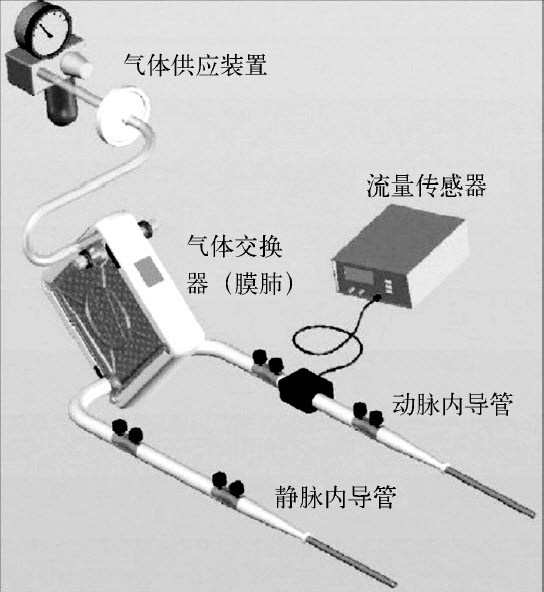
\includegraphics{./images/Image00289.jpg}
 \captionsetup{justification=centering}
 \caption{无泵的动静脉体外肺辅助系统}
 \label{fig24-2}
  \end{figure} 

\subsubsection{无泵的动静脉体外肺辅助系统的基本工作原理是什么?}

无泵的动静脉体外肺辅助系统(pECLA)是一种小容量低阻力体外膜氧合系统,与体外膜氧合相比,pECLA特点是无泵,血液灌注动力主要决定于患者动、静脉压力差,减少了泵驱动导致的血细胞破坏及凝血紊乱,减少抗凝需求,从而减少并发症,并降低治疗费用。pECLA的重要组成部分是小容量低阻膜氧合器,当血流速度为2.5L/分时,入出口之间的压力差仅15~20mmHg。氧合器材料为多聚4甲基5亚乙基六胺,膜面积1.3m\textsuperscript{2}
,预充容积250~300ml。常用动脉置管为15F~19F,静脉置管17F~19F。通常置管方式是Seldinger技术,常用部位为股动、静血管,一侧肢体选动脉置管,另一侧选静脉置管。整个系统管壁内部均包被有肝素以减少抗凝剂需要剂量。通常抗凝目标为维持激活全血凝血时间130~150秒。

pECLA的血液灌注主要由患者股动、静脉间的压差驱动,因此对于心输出量降低[CI<2.7L/(分·m\textsuperscript{2}
)]或低血压(<70mmHg)的患者不适合应用
\protect\hyperlink{text00030.htmlux5cux23ch14-29}{\textsuperscript{{[}14{]}}}
。此系统的血流量一般为0.8~2.5L/分,血流量主要影响因素是平均动脉血压和血管内置管的内径,平均动脉血压越高,血流量越大,血管内置管口径越大,血流量越大
\protect\hyperlink{text00030.htmlux5cux23ch16-29}{\textsuperscript{{[}16{]}}}
。该系统排出机体二氧化碳能力较强,即使在较低血流量(1~2.5L/分)下,排出二氧化碳的量即可占全身二氧化碳产生量的50%
\protect\hyperlink{text00030.htmlux5cux23ch6-29}{\textsuperscript{{[}6{]}}}
。此系统排出二氧化碳的能力主要由血流量和氧流量决定,为进行有效的气体交换,气体交换器需要的气体流量为10~12L/分。但此系统增加氧合的能力有限,其一是由于进入该系统内的血液(动脉)已进行了充分氧合,其次是由于血流量较小。因此,此系统的主要目的是降低动脉血二氧化碳分压,保障肺保护性通气策略的实施,预防和降低呼吸机相关肺损伤的发生
\protect\hyperlink{text00030.htmlux5cux23ch37-29}{\textsuperscript{{[}37{]}}}
。

\subsubsection{无泵的动静脉体外肺辅助系统的临床应用指征和禁忌证是什么?}

无泵的动静脉体外肺辅助系统(pECLA)是一种呼吸支持治疗手段,因此它适合于呼吸衰竭病因可逆的呼吸衰竭患者。据现有临床研究的经验,当这些呼吸衰竭患者经积极的传统治疗后氧合和(或)通气状态仍未能改善即可考虑pECLA:在呼气末正压≥10cm
H\textsubscript{2}
O的条件下,氧合指数波动于70~200mmHg之间和(或)pH<7.2
\protect\hyperlink{text00030.htmlux5cux23ch14-29}{\textsuperscript{{[}14{]}}}
。因pECLA改善氧合能力有限,对于严重的低氧血症者应进行有泵驱动的体外肺辅助技术治疗。另外,若患者存在以下的临床情况应禁止使用pECLA
\protect\hyperlink{text00030.htmlux5cux23ch3-29}{\textsuperscript{{[}3{]}}}
:严重的心功能不全患者,心输出量低于2.7L/(分·m\textsuperscript{2}
);循环不稳定,平均动脉压低于70mmHg,需要大剂量的血管活性药物[如去甲肾上腺剂量>0.4μg/(kg·分)];严重的外周血管疾病(如血栓等)和凝血紊乱患者等。

\subsubsection{无泵的动静脉体外肺辅助系统血管内置管的选择和放置注意点是什么?}

无泵的动静脉体外肺辅助系统(pECLA)血管内置管的选择和放置极为重要,是关系到pECLA临床成功实施的重要原因。在置管前,为选择合适的股动、静脉内置管,可以通过床旁血管超声评估股动、静脉的情况。动脉内导管管径要求导管置入后血管内仍有30%的剩余空间,以满足下肢的血流供应,对于亚洲人一般选择为13F~15F
\protect\hyperlink{text00030.htmlux5cux23ch15-29}{\textsuperscript{{[}15{]}}}
。静脉内导管要比动脉内导管大2F,以减少此系统对血流的阻力,增加血流量。置管时应严格按照Seldinger技术和无菌操作。置管后,应妥善安置导管和膜肺位置,防治血流量下降或反复牵拉造成穿刺部位出血,甚至导致导管不慎脱出。由于患者体位的相对固定,还需防治压疮、下肢静脉血栓等并发症。

\subsubsection{开始无泵的动静脉体外肺辅助系统后机械通气设置如何调整?}

开始无泵的动静脉体外肺辅助系统(pECLA)后应逐渐降低呼吸机参数,降低呼吸机相关肺损伤的风险。目前对于pECLA时通气参数设置未有充分的临床证据和统一标准。一般推荐以下设置方法:降低潮气量<6ml/kg、平台压<30cm
H\textsubscript{2}
O和呼吸频率<25次/分,呼气末正压按照ARDSnet研究的呼气末正压设置方法
\protect\hyperlink{text00030.htmlux5cux23ch14-29}{\textsuperscript{{[}14{]}}}
。在关于ARDS猪模型的动物研究中发现,与传统治疗方式相比,pECLA时采用近静态(near-static)通气方式(潮气量2.2ml/kg,呼气末正压15cmH\textsubscript{2}
O)能减少肺损伤的发生,包括炎性介质释放减少、表面活性物质增多和肺实质损伤减轻
\protect\hyperlink{text00030.htmlux5cux23ch39-29}{\textsuperscript{{[}39{]}}}
。另有学者建议,pECLA与高频振荡通气联合应用以进一步减少肺损伤的发生
\protect\hyperlink{text00030.htmlux5cux23ch40-29}{\textsuperscript{{[}40{]}}}
。因此,对于pECLA患者,如何选择更加保护性的通气策略有待进一步的研究证实。

\subsubsection{无泵的动静脉体外肺辅助系统过程中应注意哪些监测?}

为减少和预防无泵的动静脉体外肺辅助系统(pECLA)并发症的发生,在临床使用中还应积极地对以下主要情况进行严密监测:持续的pECLA系统血流量监测,了解系统阻力的变化;下肢血流灌注及脉氧监测,评估下肢的血供情况;凝血功能监测,避免出血和凝血的发生,首先单次给予5000IU的肝素,然后持续泵入600~800IU的肝素,滴定目标部分激活的凝血活酶时间为50~60秒或激活全血凝血时间130~150秒
\protect\hyperlink{text00030.htmlux5cux23ch38-29}{\textsuperscript{{[}38{]}}}
;为及时了解通气及氧合情况,在pECLA使用后的24小时内应每4小时监测一次血气,24小时后应每8小时监测一次;进行血液中肌酐和乳酸水平的监测,同时评估全身其他脏器的功能;另外因pECLA放置于两腿之间限制了患者的活动,还应注意预防压疮。

\subsubsection{如何撤离无泵的动静脉体外肺循环系统?}

当患者的基础原发病得到一定控制,且呼吸机支持水平显著降低(吸入氧浓度<0.5,呼气末正压<10cm
H\textsubscript{2}
O)后,即可考虑撤离无泵的动静脉体外肺循环系统(pECLA)
\protect\hyperlink{text00030.htmlux5cux23ch14-29}{\textsuperscript{{[}14{]}}}
。在撤离前,可进行自主氧合试验(spontaneous respiratory
trial,SRT)评估患者呼吸功能:将pECLA系统的氧流量降低至1L/分后,观察病人的临床反应2小时;若病人没有出现明显的气体交换和呼吸形式(如呼吸频率和分钟通气量的增加)的恶化,即可撤离此系统。拔除导管后,一定要对穿刺部位进行30分钟的持续手动摁压,然后进行24小时的持续压力绷带加压包扎,防止出血和血肿。

\subsubsection{何谓静静脉体外二氧化碳清除?}

静静脉体外二氧化碳清除(venovenous CO\textsubscript{2} removal
device,V\textsubscript{2} CO\textsubscript{2}
R)是采用双腔颈内静脉置管连接低速泵驱动的体外膜肺装置,可以采取颈内静脉单针双腔导管以较低的流速进行二氧化碳清除。基本工作原理为采用泵驱动、静脉血由双腔导管进入膜肺,二氧化碳清除后再由双腔导管另一腔回到静脉内。不存在动静脉分流,对血流动力学的影响小,避免了动脉插管造成下肢缺血的风险。虽上世纪80年代就开始临床应用于重症ARDS的治疗,但其最大流量受限,目前应用仍较少,尚未有明确的临床证据和规范。

\subsection{体外膜氧合的社会伦理及未来发展方向}

\subsubsection{体外膜氧合的家属和家庭关怀注意点是什么?}

与其他重症患者相比,体外膜氧合支持患者在很多方面具有很大不同。首先,最大的不同是接受体外膜氧合支持的患者在很长时间内几乎依赖体外膜氧合系统生存,体外膜氧合系统如果出现严重问题可直接致命;其次,患者家属已经被告知体外膜氧合是最后的拯救手段,一旦体外膜氧合不成功就几乎没有其他治疗选择,对其家人来说,在体外膜氧合支持过程中是一种心理煎熬和度日如年的过程;第三,在体外膜氧合支持下,患者的临床表现常常看起来并没有实际病情严重。患者家庭、护士、医生和体外膜氧合专门治疗人员常常会产生患者病情稳定的错觉,而对各种不良后果准备不足,因此整个抢救护理工作不仅是对患者本人的治疗,也包括对患者家庭的关怀。

患者家庭各不相同,有着不同的期望值和家庭力量,但都会表现出患者家庭成员的严重危机感和无助感。家庭成员可能很难全部理解和接受当前的各种医疗信息,可能在长时间救治患者过程中需要关怀和帮助。

如果病情允许,患者家庭应该对体外膜氧合原理有最基本的了解。应该让患者家属明白,在体外膜氧合支持状态下,尽管患者表面上看来病情改善,甚至患者处于清醒状态可正确反应,但患者自身的心肺功能可能仍然完全不工作。体外膜氧合专门人员在和患者家属沟通过程中,必须清楚表达这一重要情况。对于患者家属来说很难平衡患者恢复的希望与做好可能死亡的思想准备。患者生存的希望可以帮助家属应对目前局面,并使他们努力着眼于治疗。因此必须保持对患者家属的诚实来保持他们对危机状况的支持。如果患者出现严重并发症,或者出现不可逆的情况,被充分告知的患者家属会更有准备做出决定,撤离体外膜氧合。很多时候患者家属可能在医护人员最终确认之前就已经意识到可能继续体外生命支持已经无济于事,但每个家庭对于撤离体外膜氧合决定的反应不尽相同,必须尽可能的沟通取得家属的理解。

\subsubsection{体外膜氧合的未来发展方向是什么?}

体外膜氧合在国外的一些医疗中心已经是常规开展技术,并在不断探索其广泛临床应用。体外膜氧合适用的最佳病例、最佳时机选择、最佳辅助支持方法,体外膜氧合的撤离等仍是目前存在和需要进一步探讨的问题。随着机械材料工程等技术的发展和临床研究的深入,体外膜氧合在临床应用和实践中的未来发展方向可能在以下几个方面:

(1)对循环衰竭、呼吸衰竭、多器官功能障碍、重症感染等建立标准化治疗模式;

(2)研发优质的生物相容性材料,不易产生血栓,不需要或尽可能少使用抗凝;

(3)研发低阻力膜肺,安全高效的血泵;

(4)简单的自动化体外膜氧合设备;

(5)为早产儿提供人工胎盘;

(6)器官培养;

(7)急救复苏和器官移植或捐赠中的支持。

\begin{center}\rule{0.5\linewidth}{\linethickness}\end{center}

参考文献

\protect\hyperlink{text00030.htmlux5cux23ch1-29-back}{{[}1{]}} .Hill
JD,O'Brien TG,Murray JJ,et al.Prolonged extracorporeal oxygenation
for acute post-traumatic respiratory failure(shock-lung syndrome).Use
of the Bramson membrane lung.N Engl J Med. 1972. 286(12):629-634.

\protect\hyperlink{text00030.htmlux5cux23ch2-29-back}{{[}2{]}} .Zapol
WM,Snider MT,Hill JD,et al.Extracorporeal Membrane Oxygenation in
Severe Acute Respiratory Failure.JAMA. 1979. 242:2193-2196.

\protect\hyperlink{text00030.htmlux5cux23ch3-29-back}{{[}3{]}}
.Bartlett RH,Gazzaniga AB,Jefferies MR,et al.Extracorporeal
membraoxygenation(ECMO)cardiopulmonary support in infancy.Trans Am
Soc Artif Intern Organs. 1976. 22:80-93.

\protect\hyperlink{text00030.htmlux5cux23ch4-29-back}{{[}4{]}}
.Bindslev L.Adult ECMO performed with surface-heparinized
equipment.ASAIO Trans. 1988. 34(4):1009-1013.

\protect\hyperlink{text00030.htmlux5cux23ch5-29-back}{{[}5{]}}
.Zwischenberger JB,Nguyen TT,Upp JR Jr,et al.Complications of
neonatal extracorporeal membrane oxygenation. Collective experience
from the Extracorporeal Life Support Organization.J Thorac Cardiovasc
Surg. 1994. 107(3):838-48;discussion 848-849.

\protect\hyperlink{text00030.htmlux5cux23ch6-29-back}{{[}6{]}} .Morris
AH,Wallace CJ,Menlove RL,et al.Randomized clinical trial of
pressure-controlled inverse ratio ventilation and extracorporeal CO2
removal for adult respiratory distress syndrome.Am J Respir Crit Care
Med. 1994. 149(2 Pt 1):295-305.

\protect\hyperlink{text00030.htmlux5cux23ch7-29-back}{{[}7{]}} .Zapol
WM,Snider MT,Hill JD,et al.Extracorporeal membrane oxygenation in
severe acute respiratory failure.A randomized prospective study.JAMA.
1979. 242(20):2193-2196.

\protect\hyperlink{text00030.htmlux5cux23ch8-29-back}{{[}8{]}} .Peek
GJ,Mugford M,Tiruvoipati R,et al.Efficacy and economic assessment of
conventional ventilatory support versus extracorporeal membrane
oxygenation for severe adult respiratory failure(CESAR):a multicentre
randomised controlled trial.Lancet. 2009. 374(9698):1351-1363.

\protect\hyperlink{text00030.htmlux5cux23ch9-29-back}{{[}9{]}} .Davies
A,Jones D,Bailey M,et al.Extracorporeal Membrane Oxygenation for
2009 Influenza A(H1N1)Acute Respiratory Distress Syndrome.JAMA. 2009.
302(17):1888-1895.

\protect\hyperlink{text00030.htmlux5cux23ch10-29-back}{{[}10{]}} .Noah
MA,Peek GJ,Finney SJ,et al.Referral to an extracorporeal membrane
oxygenation center and mortality among patients with severe 2009
influenza A(H1N1).JAMA. 2011. 306(15):1659-1668.

\protect\hyperlink{text00030.htmlux5cux23ch11-29-back}{{[}11{]}}
.Brodie D,Bacchetta M.Extracorporeal membrane oxygenation for ARDS in
adults.N Engl J Med. 2011. 365(20):1905-1914.

\protect\hyperlink{text00030.htmlux5cux23ch12-29-back}{{[}12{]}}
.Checkley W.Extracorporeal membrane oxygenation as a first-line
treatment strategy for ARDS:is the evidence sufficiently strong.JAMA.
2011. 306(15):1703-1704.

\protect\hyperlink{text00030.htmlux5cux23ch13-29-back}{{[}13{]}}
.Schuerer DJ,Kolovos NS,Boyd KV,et al.Extracorporeal membrane
oxygenation:current clinical practice,coding,and
reimbursement.Chest,2008,134:179-184.

\protect\hyperlink{text00030.htmlux5cux23ch14-29-back}{{[}14{]}}
.Zimmermann M,Bein T,Arlt M,et al.Pumpless extracorporeal
interventional lung assist in patients with acuterespiratory distress
syndrome:a prospective pilot study.Crit Care. 2009. 13(1):R10.

\protect\hyperlink{text00030.htmlux5cux23ch15-29-back}{{[}15{]}} .Bein
T,Weber F,Philipp A,et al.A new pumpless extracorporeal
interventional lung assist in critical hypoxemia/hypercapnia.Crit Care
Med. 2006. 34(5):1372-1377.

\protect\hyperlink{text00030.htmlux5cux23ch16-29-back}{{[}16{]}}
.Muller T,Lubnow M,Philipp A,et al.Extracorporeal pumpless
interventional lung assist in clinical practice:determinants of
efficacy.Eur Respir J. 2009. 33(3):551-558.

\protect\hyperlink{text00030.htmlux5cux23ch17-29-back}{{[}17{]}}
.Nierhaus A,Frings D,Braune S,et al.Interventional lung assist
enables lung protective mechanical ventilation inacute respiratory
distress syndrome.Minerva Anestesiol. 2011. 77(8):797-801.

\protect\hyperlink{text00030.htmlux5cux23ch18-29-back}{{[}18{]}}
.Gattinoni L,Pesenti A,Mascheroni D,et al.Low-frequency
positive-pressure ventilation with extracorporeal CO2 removal insevere
acute respiratory failure.JAMA. 1986. 256(7):881-886.

\protect\hyperlink{text00030.htmlux5cux23ch19-29-back}{{[}19{]}}
.Batchinsky AI,Jordan BS,Regn D,et al.Respiratory
dialysis:reduction in dependence on mechanical ventilation byvenovenous
extracorporeal CO\textsubscript{2} removal.Crit Care Med. 2011.
39(6):1382-1387.

\protect\hyperlink{text00030.htmlux5cux23ch20-29-back}{{[}20{]}}
.Cardenas VJ Jr,Miller L,Lynch JE,et al.Percutaneous venovenous
CO\textsubscript{2} removal with regional anticoagulation in an
ovinemodel.ASAIO J. 2006. 52(4):467-470.

\protect\hyperlink{text00030.htmlux5cux23ch21-29-back}{{[}21{]}} .Doll
N,Kiaii B,Borger M,et al.Five-year results of 219 consecutive
patients treated with extracorporeal membrane oxygenation for refractory
postoperative cardiogenic shock.Ann Thorac Surg. 2004.
77(1):151-157;discussion 157.

{[}22{]}.Elsharkawy HA,Li L,Esa WA,et al. Outcome in patients who
require venoarterial extracorporeal membrane oxygenation support after
cardiac surgery.J Cardiothorac Vasc Anesth. 2010. 24(6):946-951.

\protect\hyperlink{text00030.htmlux5cux23ch23-29-back}{{[}23{]}} .Kumar
TK,Zurakowski D,Dalton H,et al.Extracorporeal membrane oxygenation
in postcardiotomy patients:factors influencing outcome.J Thorac
Cardiovasc Surg. 2010. 140(2):330-336.e2.

\protect\hyperlink{text00030.htmlux5cux23ch24-29-back}{{[}24{]}} .Acker
MA.Mechanical circulatory support for patients with acute-fulminant
myocarditis.Ann Thorac Surg. 2001. 71(3 Suppl):S73-76;discussion
S82-85.

\protect\hyperlink{text00030.htmlux5cux23ch25-29-back}{{[}25{]}}
.Kawahito K,Murata S,Adachi H,et al.Resuscitation and circulatory
support using extracorporeal membrane oxygenation for fulminant
pulmonary embolism.Artif Organs. 2000. 24(6):427-430.

\protect\hyperlink{text00030.htmlux5cux23ch26-29-back}{{[}26{]}} .Chen
YS,Lin JW,Yu HY,et al.Cardiopulmonary resuscitation with assisted
extracorporeal life-support versus conventional cardiopulmonary
resuscitation in adults with in-hospital cardiac arrest:an
observational study and propensity analysis.Lancet. 2008.
372(9638):554-561.

\protect\hyperlink{text00030.htmlux5cux23ch27-29-back}{{[}27{]}} .Baud
FJ,Megarbane B,Deye N,Leprince P. Clinical review:aggressive
management and extracorporeal support for drug-induced
cardiotoxicity.Crit Care. 2007. 11(2):207.

\protect\hyperlink{text00030.htmlux5cux23ch28-29-back}{{[}28{]}}
.Watson WA,Litovitz TL,Klein-Schwartz W,et al. 2003 annual report of
the American Association of Poison Control Centers Toxic Exposure
Surveillance System.Am J Emerg Med. 2004. 22(5):335-404.

\protect\hyperlink{text00030.htmlux5cux23ch29-29-back}{{[}29{]}}
.Fortenberry JD,Paden ML.Extracorporeal therapies in the treatment of
sepsis:experience and promise.Semin Pediatr Infect Dis. 2006.
17(2):72-79.

\protect\hyperlink{text00030.htmlux5cux23ch30-29-back}{{[}30{]}} .Vohra
HA,Adamson L,Weeden DF,Haw MP.Use of extracorporeal membrane
oxygenation in the management of septic shock with severe cardiac
dysfunction after Ravitch procedure.Ann Thorac Surg. 2009.
87(1):e4-5.

\protect\hyperlink{text00030.htmlux5cux23ch31-29-back}{{[}31{]}} .Li
J,Long C,Lou S,et al.Venoarterial extracorporeal membrane
oxygenation in adult patients:predictors of mortality.Perfusion. 2009.
24(4):225-230.

\protect\hyperlink{text00030.htmlux5cux23ch32-29-back}{{[}32{]}}
.龙村.当今体外膜肺氧合趋势和对中国的几点建议.中国体外循环杂志. 2010.
8(1):1-3.

\protect\hyperlink{text00030.htmlux5cux23ch33-29-back}{{[}33{]}}
.Mottaghy K,Oedekoven B,Poppel K,et al.Heparin free long-term
extracorporeal circulation using bioactive surfaces.ASAIO Trans. 1989.
35(3):635-637.

\protect\hyperlink{text00030.htmlux5cux23ch34-29-back}{{[}34{]}} .Plotz
FB,van OW,Bartlett RH,Wildevuur CR.Blood activation during neonatal
extracorporeal life support.J Thorac Cardiovasc Surg. 1993.
105(5):823-832.

\protect\hyperlink{text00030.htmlux5cux23ch35-29-back}{{[}35{]}}
.Hocker JR,Wellhausen SR,Ward RA,et al.Effect of extracorporeal
membrane oxygenation on leukocyte function in neonates.Artif Organs.
1991. 15(1):23-28.

\protect\hyperlink{text00030.htmlux5cux23ch36-29-back}{{[}36{]}}
.Robinson TM,Kickler TS,Walker LK,et al.Effect of extracorporeal
membrane oxygenation on platelets in newborns.Crit Care Med. 1993.
21(7):1029-1034.

\protect\hyperlink{text00030.htmlux5cux23ch37-29-back}{{[}37{]}}
.Moerer O,Quintel M.Protective and ultra-protective
ventilation:using pumpless interventional lungassist(iLA).Minerva
Anestesiol. 2011. 77(5):537-544.

\protect\hyperlink{text00030.htmlux5cux23ch38-29-back}{{[}38{]}} .Hamid
IA,Hariharan AS,Shankar NR.The advent of ECMO and pumpless
extracorporeal lung assist in ARDS.J Emerg Trauma Shock. 2011.
4(2):244-250.

\protect\hyperlink{text00030.htmlux5cux23ch39-29-back}{{[}39{]}}
.Iglesias M,Jungebluth P,Petit C,et al.Extracorporeal lung membrane
provides better lung protection than conventionaltreatment for severe
postpneumonectomy noncardiogenic acute respiratory distress syndrome.J
Thorac Cardiovasc Surg. 2008. 135(6):1362-1371.

\protect\hyperlink{text00030.htmlux5cux23ch40-29-back}{{[}40{]}}
.Kredel M,Brederlau J,Wunder C,et al.High-frequency oscillatory
ventilation with and without arteriovenousextracorporeal lung assist in
patients with severe respiratory failure.J Crit Care. 2011.

\protect\hypertarget{text00031.html}{}{}

